\documentclass[12pt,a4paper]{report}
\usepackage{graphicx} % For including images
\usepackage{tocloft} % Optional: Customize the table of contents
\usepackage[a4paper, margin=2cm]{geometry} % Adjust margin 
\usepackage{hyperref} % enables hyperlinks
\hypersetup{
    colorlinks=true,        % Enables colored links
    linkcolor=blue,         % Color of internal links (e.g., table of contents)
    citecolor=blue,         % Color of citation links
    filecolor=magenta,      % Color of file links
    urlcolor=blue           % Color of external links
}
\usepackage{cite} %betterhandling of citation
\setcounter{secnumdepth}{3} % Allows subsubsections to be numbered
\setcounter{tocdepth}{3} % Includes up to subsubsections in the TOC
\usepackage{xcolor}
\definecolor{darkblue}{RGB}{0,0,139} % Dark blue color
\usepackage{booktabs}
\usepackage{wrapfig}



% For the R codes
\usepackage{listings}
\usepackage{xcolor}

\lstdefinestyle{mystyle}{
    backgroundcolor=\color{white},   % background color
    basicstyle=\ttfamily\small,      % font style and size
    keywordstyle=\color{blue},       % keyword color
    commentstyle=\color{gray},       % comment color
    stringstyle=\color{red},         % string color
    showstringspaces=false,          % don't show space symbols
    numbers=none,                    % line numbers
    numberstyle=\tiny\color{gray},   % line number style
    stepnumber=1,                    % step between two line numbers
    numbersep=5pt,                   % how far the line numbers are from the code
    frame=single,                    % add a frame around the code
    rulecolor=\color{black},         % frame color
    breaklines=true                  % automatically break lines
}

\begin{document}
\begin{titlepage}
    \centering
    \begin{flushright}
        \centering
        
\includegraphics[width=2cm]{images/thd.png} % Adjust width as needed
        \hspace{0cm} % Space between images
        
\includegraphics[width=2cm]{images/ipb.jpg} % Adjust width as needed
    \end{flushright}
    {\huge\bfseries Development of an R Toolbox for Near-Infrared Spectroscopy Data Processing \\
    and Analysis of Plant Metabolic Phenotypes\par}
    \vspace{2cm}
    {\LARGE \textsc{Deggendorf Institute of Technology}\par}
    \vspace{1cm}
    {\Large \textsc{MSc. Life Science Informatics}\par}
    \vspace{1.5cm}
    {\Large\itshape Methun George\par}
    \vfill
    Supervised by\par
    PD Dr. habil. rer. nat. Steffen Neumann\par
    Prof. Dr. Melanie Kappelmann-Fenzl
    \vfill
    {\large \today\par}
\end{titlepage}

% --------------Acknowledgement section---------------------
\newpage
\section*{Acknowledgements}
This Master Thesis has been an incredibly enjoyable experience. In pursuit of my passion for bioinformatics and molecular biology, this master’s thesis project has been a profoundly enriching journey. It offered me an incredible platform to implement the knowledge I gained in various programming languages and bioinformatics tools during my master’s studies along with the knowledge of botany I gained from my bachelor degree. This thesis not only deepened my technical expertise but also provided an invaluable opportunity to explore the practical applications of these skills in real-world research. \\

I am deeply indebted to my supervisor, Dr. Steffen Neumann, at the Leibniz Institute of Plant Biochemistry (IPB Halle), for his unwavering support, insightful guidance, and expert advice. The mentorship of Dr. Neumann played a great role in navigating the complexities of this project and sharpening my understanding of computational approaches in plant biology. Thank you for making this possible and for the always open door. \\

I express my heartfelt gratitude to my professor, Dr. Melanie Kappelmann-Fenzl, at the Technische Hochschule Deggendorf (THD), for her academic guidance and constant encouragement throughout my master’s degree. Her feedback and insights were instrumental in shaping the direction and quality of my research. \\

I am profoundly grateful to the Computational Plant Biochemistry (CPB) and MetaCom team at IPB Halle, especially Dr. Henriette Uthe, Dr. Rene Meier, Dr. Michael Wenk, Oliver Duchrow, Dr. Khabat Vahabi, and Norman Storz, whose expertise and assistance greatly enriched my learning experience. Their collaborative spirit and support made this research endeavor not only productive but also highly inspiring. \\

My deepest gratitude goes to my family and friends, whose unending love, unwavering support, and endless encouragement have been my foundation throughout this journey. Their belief in me has been the source of my strength and motivation. \\

Lastly, I would like to express my sincere appreciation to all the faculty members of the Life Science Informatics program at the Technische Hochschule Deggendorf and all the members in Leibniz-Institute for Plant Biochemistry. Their guidance and encouragement at various stages of my degree have been invaluable. \\

This thesis is a culmination of the collective support and encouragement that I have received from all these individuals and institutions, and I am ever grateful for their contributions to my academic and professional growth. \\

%----------------Abstract page------------------------------------
\newpage
\section*{Abstract}
The abstract of this thesis is..................................

% ----------------Table of contents---------------------------------
\newpage
\tableofcontents

% ---------------Abbreviations-------------------------------------
\newpage
\section*{Abbreviations}
\begin{tabbing}
    \textbf{Abbreviation} \hspace{2cm} \= \textbf{Full Form} \\
    \\
    NIRS \> Near Infrared Spectroscopy \\
    LC-MS \> Liquid Chromatography Mass Spectroscopy \\
    CNN \> Convolutional Neural Network \\
    DL \> Deep Learning \\
    PLSR \> Partial Least Squares Regression \\
    PCA \> Principal Component Analysis \\
    ML \> Machine Learning \\
    NIRS \> Near-Infrared Spectroscopy \\
    SLA \> Specific Leaf Area \\
    RF \> Random Forest \\
    SLA \> Specific Leaf Area \\
    LDMC \> Lead Dry Matter Content \\
    R\textsuperscript{2} \> Coefficient of Determination \\
    ADAM \> Adaptive Moment Estimation \\
    SGD \> Stochastic-Gradient Descent \\
    AdaGrad \> Adaptive Gradient Algorithm \\
    RMSProp \> Root Mean Square Propagation \\
    MSC \> Multiplicative Scatter Correction \\
    SNV \> Standard Normal Variate \\
    GMO \> Genetically Modified Organisms \\
    HCA \> Hierarchical Cluster Analysis \\
    PLSDA  \> Partial Least Squares Discriminant Analysis \\
    ANA \>  Artificial Neural Network \\
    LDA \> Linear Discriminant Analysis \\
    RNN \> Recurrent Neural Network \\
    CRAN \> Comprehensive R Archive Network \\
    LC \> Liquid Chromatography \\
    RT \> Retention Time \\
    
\end{tabbing}

%---------------Chapters and Sections----------------------------------------------------
\chapter{Introduction}
The understanding of interplay between plant physiology and its hidden biochemical process is crucial for the improvement of basic plant science and addressing global challenges such as food security, crop resilience and combating climate change [1]. 
In recent years, advanced High-throughput analytical techniques such as Near-Infrared Spectroscopy (NIRS) and Liquid Chromatography-Mass Spectrometry (LC-MS) has instigated a paradigm shift in plant biology [2,3].
These High-throughput techniques are mostly used in areas like genomics, imaging and spectroscopy and are known for their ability to collect and analyse the data faster than traditional techniques[3].
High-throughput techniques are widely used since they enable the efficient collection of vast amount of data at various scales, from molecular to field level over significant time periods[4].
The big data generated by these high throughput procedures present both opportunities and challenges at the same time. It requires efficient processing to extract the maximum useful results and this is where Machine Learning (ML) or Deep Learning (DL) becomes indispensable [4,5].
ML as part of Artificial Intelligence (AI) refers to the ability of computers to find patterns and learn from existing data, which can be employed in processing high-dimensional data [6,4]. The ML algorithms are powerful enough to analyse complex, high dimensional datasets, 
enabling accurate predictions of plant traits or other features based on the input data. Additionally, integrating these big data with ML could help the researchers to optimize data processing pipelines, enhance predictive accuracy and thereby enter into a new era of data-driven decision-making [4,5]. This project employs linear model, non-linear model and neural networks to predict various plant features and compare their predictive accuracy, error rate and training time. \\


A significant  shift in the realm of the biomedical community has brought new guidelines to ensure readability, modularity, transparency and extensibility of computational toolboxes. A toolbox, which stores multiple functions, parameters and results in a central location should be maintainable and uncomplicated for the developers and members of the open-source community [7].
R is a powerful and widely used programming language in the analysis and processing of high throughput data. Additionally, R contains a multitude of statistical and high quality visualization packages such as ggplot2 which are capable of processing and integrating big data to different ML methods [8]. Bioconductor is an open source software for bioinformatics, which contains more than 3691 packages (according to the last update in 2024) for statistical computing. 
This offers an object oriented framework for the high dimensional data, cutting edge visualization capabilities and interoperability [9]. Existing tools in Near-Infrared Spectroscopy (NIRS) data processing lack functionalities that could simplify and standardize data workflows when integrated with the SummarizedExperiment framework from the Bioconductor package. To address these gaps, the R toolbox, “nearspectRa” was developed for processing NIRS data.
This package has a modular structure which creates a SummarizedExperiment object from NIRS data. \\


Metabolomics, the study of small molecular compounds in biological systems, is a rapidly advancing field of science with applications in biotechnology, medicine, synthetic biology and environmental science [6]. Metabolomics has emerged as a transformative tool in plant biology, enabling cost-efficient and high throughput molecular characterization.
The integration of metabolomics with different omics approaches has proven invaluable for functional genes identification and developing trait specific markers [10]. Metabolomics, which is built on the advancement of phenomics and genomics, provides high throughput and precise profiling of metabolites, revealing the physiological state of cells [6,10].
Metabolites play a crucial role in plant metabolism, influencing its biomass and architecture therefore study of these small molecules will aid in uncovering plant regulatory mechanisms and pathway interactions [10].
The coupling of liquid or gas chromatography with mass spectrometry or nuclear magnetic resonance spectroscopy (NMR) facilitates measurement of thousands of metabolites, thereby providing a comprehensive view of biochemical and biological mechanisms [11]. Therefore, Mass spectrometry(MS) remains the most widely used analytical approach among others due to its versatility and sensitivity [6].
Mass spectrometry based metabolomics generate data of high sensitivity and throughput requiring advanced computational methods. Machine learning not only offers a powerful solution to analyse such data, but also helps in resolving the challenges like noise, batch effects and missing values [12]. Integrating ML with Liquid Chromatography-Mass Spectroscopy (LC-MS) data helps us to analyse this complex heterogeneous data rapidly, enabling deeper insights. \\


Near-Infrared Spectroscopy (NIRS) is an advanced high throughput and non-destructive analytical technique that uses light in the near-infrared region (780-2500 nm) to assess the chemical composition of samples [13]. The light is either absorbed or reflected by the sample at different wavelengths and thereby creating a spectrum[13]. The NIRS is widely used in plant research due to its ability in predicting sample structure and traits by analysing the spectral patterns.
NIRS can also be used in the quantitative analysis of key plant features such as protein and carbohydrate content, secondary metabolites and physiological traits such as Specific Leaf Area (SLA) by developing calibration models between spectra and reflectance trait data [14,13]. NIRS is not only used in plant biology but also in various fields such as food science, agriculture and pharmaceuticals. When compared to other analytical techniques, NIRS is rapid, 
requires minimal sample preparation and less expensive, which makes it more attractive and interesting to the scientific communities [13]. However, on the flip side it requires complex statistical methods to extract different complex features due to the highly-correlated nature of NIRS data [13]. To tackle this problem, the conventional methods such as Partial Least Square Regression (PLSR) and Principal Component Analysis (PCA) imply dimension reduction which 
result in loss of information and often struggles to extract important features from the spectral data [13]. To address the challenge of data complexity and generalizability, different ML methods can be used to predict the traits from the NIRS data [13,15]. In this project different ML and Deep Learning (DL) has been employed to predict different plant leaf traits with use of NIRS data. \\


In recent years, studies using NIRS data coupled with PLSR have been used as an alternative for traditional methods such as high-performance liquid chromatography (HPLC) and mass spectrometry which are both labor-intensive and expensive to predict different plant traits. A notable example is the prediction of glucobrassicin (GBS) concentrations from NIRS data. This has shown that GBS 
concentrations could be reliably predicted from NIRS data [16]. Another prominent example is the tree and mycorrhizal fungal diversity experiment and  trait variation in temperate forests  conducted by Pablo Castro Sanchez-Bermejo, where he combined Deep Learning (DL) approaches with leaf-level spectral data to predict 5 different leaf traits [15]. Another good  example is a 
project involving the development of white-box  workflow for regression tasks [17]. The project marks the potential of Regression (Sensitive) Neural Gas (RSNG) for generating interpretable results while maintaining high accuracy [17]. From the above studies, it is evident that NIRS data has a wide range of applications in plant research. This can also be expanded further to predict 
complex metabolites which are usually assessed via techniques like LC-MS. Moreover, integrating NIRS with advanced ML could further enhance the prediction accuracy and unlock new possibilities in plant science. \\


The past decade has witnessed the increasing popularity of  Artificial Intelligence (AI) in different fields. However, this idea of AI has been under development since 1956, starting from the concept of “programming computers to think and reason” [18]. In other words, AI can be described as “automating intellectual tasks normally done by humans” [18]. Machine learning (ML) and Deep learning (DL) are the methods that fall under the realm of AI [18,19]. 
Nowadays, there are different ML algorithms in use, in which the most popular ones include Partial Least Square Regression (PLSR), Random Forest (RF) and Convolutional Neural Network (CNN) [20,18]. PLSR is a linear and one of the most simple ML approach. It uses the advantages of PCA and linear regression to solve the regression problem in the high dimensional data [18]. On the other hand,  Random forest is a non-linear approach in ML that is primarily used for classification. It can also 
be used for regression tasks and can be represented as a decision tree with a series of nodes starting from a root node. The terminal node will predict the class of data in classification tasks [18]. For regression tasks, the random forest works differently compared to classification but the core principles remains the same. The terminal node of RF in regression takes the avarage of predictions from the individual trees [44]. The Convolutional neural networks are a specialized type of neural network which are mainly used in the field of image processing [21]. A recent study of mycorrhizal fungal diversity experiment and  trait variation in temperate forests  conducted by Pablo Castro Sanchez-Bermejo, 
demonstrated the application of CNN in predicting the leaf trait values from NIRS data, achieving superior results [15]. This outcome strongly suggests the potential of CNN not only for classification tasks such as image processing but also for regression tasks. In another project, CNN was used to predict gene expression status on the basis of sequence of gene transcription start regions. The CNN model had achieved roughly 80\% accuracy [22]. 
These studies highlight the growing versatility of CNN models. \\


Omics is a term associated with the field of large scale biological data, including genomics, epigenomics, proteomics, transcriptomics and metabolomics [23]. Combination of data from these techniques along with advanced microscopy techniques helps in the study of biomolecules in cellular and subcellular levels [23]. However, the high throughput data from these omics instruments poses challenges in processing and analysing it without the loss of information [23,10]. 
The complexity and scale of this data make ML essential for effective integration and analysis, raising the critical question: which ML model is best suited to handle this data? How much programming expertise is necessary to implement these models? And, which models are most suitable for regression tasks?. Each ML model handles the data differently. For instance, PLSR uses latent variables to capture the covariance between predictor and response variables. Moreover, 
PLSR uses the combination of Principal Component Analysis (PCA) and linear regression [20]. In the case of RF, it follows the concept of “a forest made of many trees” which uses the combination of predictions from many trees [18]. Among these ML techniques, CNN is gaining attention on its ability in handling high throughput data and predicting with remarkable accuracy [15,22]. These ML models also require different levels of programming proficiency and computational resources, depending on the scale of data. \\


In the light of the findings, it is clear that ML can significantly improve the analysis and processing of high throughput data from analytical techniques such as LC-MS and NIRS [15,22,17]. Among these, NIRS stands out as a non-destructive, cost-effective and rapid method, offering valuable insights into the chemical composition of the biological samples [12,13,14]. These qualities make NIRS a promising technique to optimize and integrate with ML and DL models for predictive accuracy. \\


Given the popularity of R programming within the ecological and bioinformatic community, it was chosen as the foundation for this project [7,9]. Recognizing the need for specialized tools to process the NIRS data, an R package, nearspectRa, was developed to handle data from two widely used NIRs instruments namely “ASD Fieldspec 4” and Spectra Vista Corporation (SVC) HR-1024i. 
Leveraging supporting packages like “R-FieldSpectra”, the high dimensional data was structured into a “SummarizedExperiment” object, aligning with Bioconductor standards for interoperability and integration. \\


Apart from developing a Good Scientific Practice (GSP) compliant package, this project involved two key analyses: first, predicting plant leaf traits from NIRS data using three popular ML methods, PLSR, RF and CNN and second predicting LC-MS features from NIRS data using the same models. To evaluate these approaches, performance was compared using metrics such as the coefficient of determination ($R^2$), Root Mean Squared Error (RMSE) and training time of each model. Additionally,
extrapolation studies were conducted on PLSR and RF to assess the robustness and performance of those beyond training data. This project not only exemplifies good scientific practice in developing an R toolbox but also provides a comprehensive comparison of linear, non-linear and neural network based NL approaches in predicting plant traits and LC-MS features from NIRS data. By achieving this, the project makes a significant milestone, paving the way for a new era of cost-effective, rapid biochemical analysis in metabolomics. \\


%--------------------------------Background--------------------------------------------------

\chapter{Background}

\section{Near Infrared Spectroscopy (NIRS)}
Near infrared spectroscopy (NIRS) is a non-invasive measurement technique that uses light in
the near infrared region to analyse a sample [35,13]. Infrared (IR) is a form of electromagnetic
radiation and it interacts with samples through absorption or reflection. The NIRS is widely
used in plant research due to its ability in predicting sample structure and traits by analysing
the spectral patterns. Based on how the sample absorbs or reflects light at different wavelengths, Infrared radiation is classified into three categories:(1) Near Infrared (NIR), ranging from 780 to 2500 nanometers (nm), (2) Mid Infrared (MIR),ranging from 2500 to 25,000 nm, and (3) Far Infrared (FIR), ranging from 25,000 to 1,000,000nm [35]. When a substance such as plant leaf is subjected to NIR light, the molecular bonds in the infrared range will interact with the light thereby causing absorption or reflection of light by the sample. The light transmitted or reflected is then measured to produce the NIR spectrum. This spectrum provides a detailed picture of molecular composition of the substance and the peaks in the spectrum corresponding to different vibrational modes of different chemical bonds. This occurs due to the change in the vibrational or rotational state of molecules or transition between their energy levels [35,13]. The group which is the most dominant in absorbing the NIR are hydrogen-containing groups such as C-H, O-H and N-H while other groups like C=C and C=O absorbs light in weaker intensities. These groups are key components in organic substances and their absorption wavelengths and intensities differ depending on the chemical composition of the substance [35].
  \\ 

\begin{figure}[h]
    \centering
    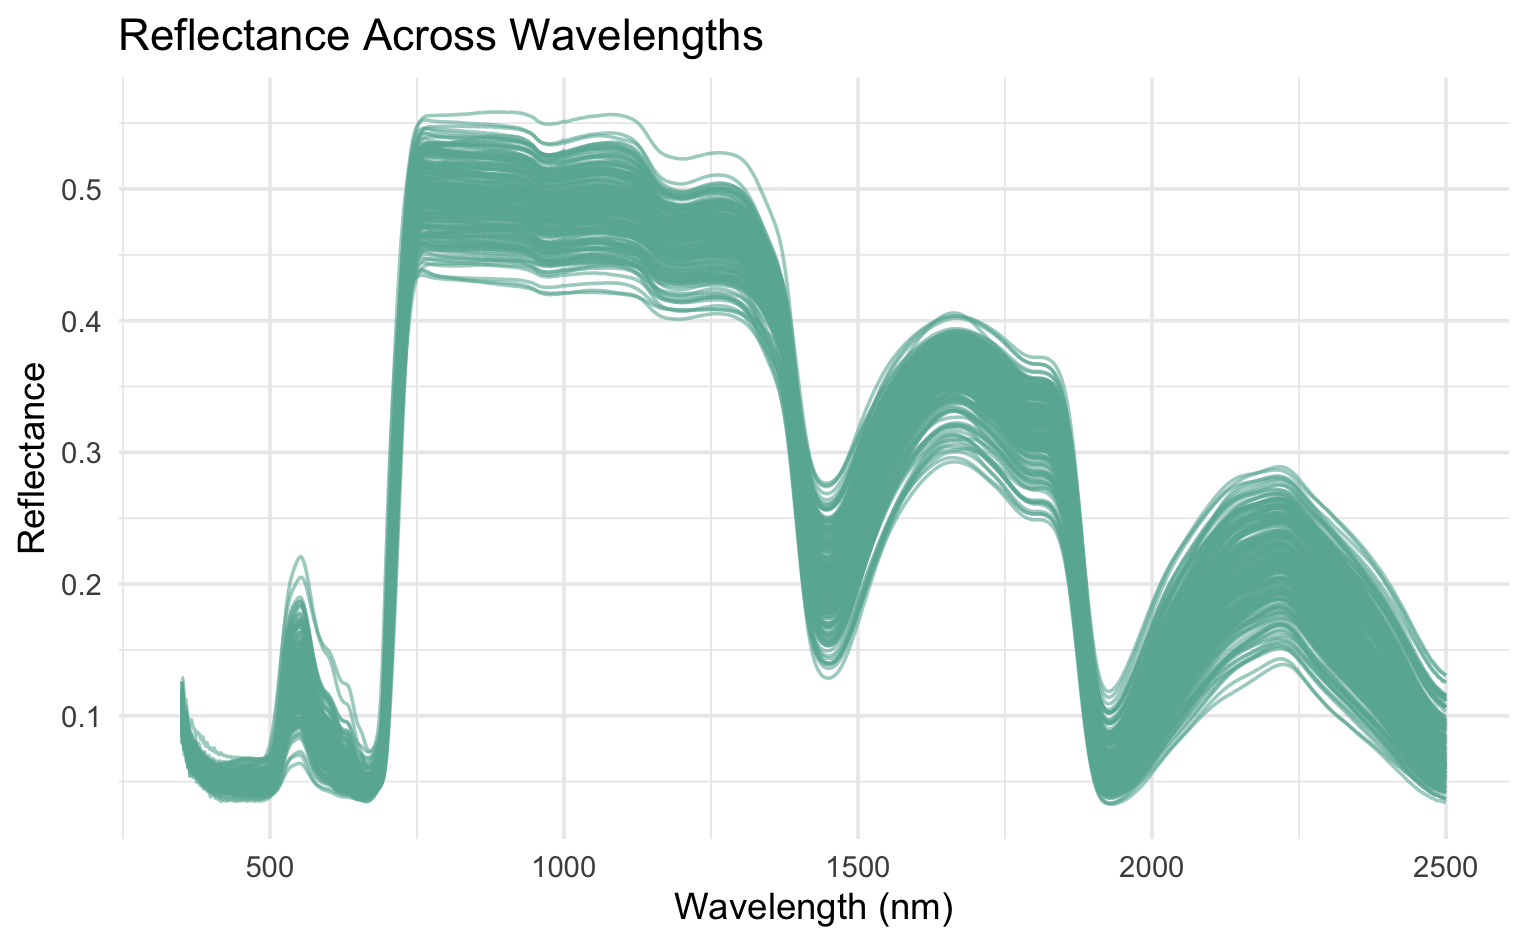
\includegraphics[width=0.8\textwidth]{images/NIRS_spectra.png} 
    \caption{Example near-infrared spectra illustrating reflectance across wavelengths. Each line represents a unique sample, showing how NIRS captures molecular absorption/reflectance patterns.}
    \label{fig:nirs_spectra}
\end{figure}

The figure \ref{fig:nirs_spectra} cite an example of the relationship between reflectance and wavelength for
near-infrared (NIR) spectra where the variations in reflectance give valuable information
about the chemical and physical properties of the sample. Compared to other analytical meth-
ods, NIRS is faster, requires little sample preparation, and is more cost-effective, making it a
highly inviting choice for researchers and scientists [13]. NIR spectrometers typically consist
of a light source, a beam splitter, optical detectors and optionally a processing system or a
monitor. The components differ depending on the purpose of the instrument to make sure accuracy
and consistency. These systems can operate in different modes such as transmission, reflection,
diffuse reflectance or transfectance depending on the type of analysis [36]. The collected spectra
will be later put through chemometric analysis to develop a calibration model using key NIR
bands. Nevertheless, NIRS require reference data from traditional chemical analysis for accurate
quantitative analysis [36]. The spectra are usually exposed to preprocessing to remove irrelevant information to improve the accuracy of the analysis. The most common preprocessing techniques
include, baseline correction, scatter correction, noise removal and wavelength selection. The
scatter correction method and spectral derivatives are the most used preprocessing approaches
in NIRS. The scatter correction method includes, Multiplicative scatter correction (MSC) and
Standard normal variate (SNV). Additionally a wide range of normalization methods such as
mean centering, auto scaling, vector normalization and area normalization are also used in pre-
processing of NIRS data. The preprocessing methods are aimed to highlight important spectral
features but must be carefully selected to avoid losing critical information [36]. \\

NIRS consist of overlapping weak bands that require multivariate calibration for quantitative analysis. These methods analyze the data in a way that can identify patterns or make predictions [36]. Techniques like Principal component analysis (PCA), Partial least squares discriminant analysis (PLSDA), Hierarchical cluster analysis (HCA) and Linear discriminant analysis (LDA) are used for classification, while others like Artificial neural networks (ANNs) handle more complex relationships. 
Deep learning (DL) is a subset of ML that has a wide range of applications including image and audio recognition [36]. ML can also be used in the handling of “Big Data” emerging from the growing spectral libraries. DL models, unlike the traditional neural networks, consist of multiple layers to extract different features from the data resulting in better predictions [36]. In recent years techniques like Convolutional neural network (CNN), recurrent neural network (RNN) and DeepSpectra 
model have gained popularity. Combining DL with spectroscopy shows a great promise in applications like food quality assessment and genetically modified organisms (GMO) detection [36].\\

The NIRS has diverse biological applications, particularly in agricultural and soil sciences. In recent years, it has been employed to analyse the crops, food properties and plant traits, including water content, pH, oil, protein, and fatty acids. Another example would be the use of NIRS to predict anthocyanin levels in grapes and black rice seeds. Researchers have also used NIRS to identify pest attacks and pesticide residues in crops making it invaluable for quality assessment 
in agriculture [36]. Even Though, much of the NIRS applications focused on agriculture and food quality, its applications in food safety are also growing. For instance,NIRS can effectively evaluate the lamb meat tenderness, pH, fat and water content. The portable NIRS devices allow real time industrial monitoring making it suitable for large scale monitoring of meat, fruits, vegetables and beverages for quality and safety [36]. Genetically modified organisms (GMO) pose a risk of 
gene transfer, which could threaten environmental biodiversity. NIRS has shown potential for rapid and cost effective GMO detection in labs and fields, making it a favored tool among researchers for monitoring GMOs [36]. \\

\paragraph{\textbf{\textcolor{darkblue}{NIRS Instruments}}}
The ASD FieldSpec4 and SpectraVista Corporation (SVC) HR-1024i are two widely used NIRS instruments in plant biology are highly relevant to this project. \\

\textcolor{darkblue}{ASD FieldSpec4}\\
ASD FieldSpec4 is a portable NIRS instrument produced by  Malvern panalytical and comes in different variants. It has a wide range of applications including, plant physiology, remote sensing and geology, atmospheric remote sensing research and biomass analysis among others. It provides data across the wavelength of 350 to 2500 nm. There are multiple optional accessories, contact probe (contact measurements like solid raw materials, grains, other granular materials), reflectance panels, pistol grips and leaf clip version 2 are few out of many [40]. \\
\\
\textcolor{darkblue}{SVC HR-1024i}\\
This is a high resolution portable spectroradiometer which provides data across a full spectral region from 350 to 2500 nm. Compared to ASD FieldSpec4, SVC HR-1024i comes with a built-in touch screen to set parameters and review data in real time, which makes it more advanced. It is also light weight and has an internal GPS and a camera which adds critical information to the spectral signature. The output from this instrument is human readable and easy to interpret without the use of any package [41]. \\


\section{Liquid Chromatography Mass Spectrometry}
Liquid Chromatography-Mass Spectrometry(LCMS) is the combination of two powerful analytical techniques for the separation, identification and quantification of biological compounds from complex mixtures. This technique has a wide range of applications in Metabolomics, Pharmaceuticals, environmental science and food chemistry [43]. Liquid Chromatography (LC) 
is a technique used to separate components in a mixture based on the rates at which they move through a stationary phase under the influence of mobile phase gradient. The varying affinities of the components to the stationary and mobile phases leads to their separation, with some attached to the mobile phase and eluting faster, while others attach to 
the stationary phase and thereby elute more slowly, leading to different retention times (RT) [43]. Mass spectrometry (MS) is one of the several detectors which can be coupled with LC to identify compounds. MS detects the mass to charge ratio (m/z) and the abundance of ions generated during ionization of the sample extracts [43]. Ions are charged molecules 
and are easier to analyze than neutral molecules therefore ionization is a crucial step in MS [43]. The MS is made of an ionization source, a mass analyzer and a detector, all these should be kept under vacuum to optimize the ion transmission. A mass spectrum is then generated with the help of a computer [43]. \\

\begin{figure}[h]
    \centering
    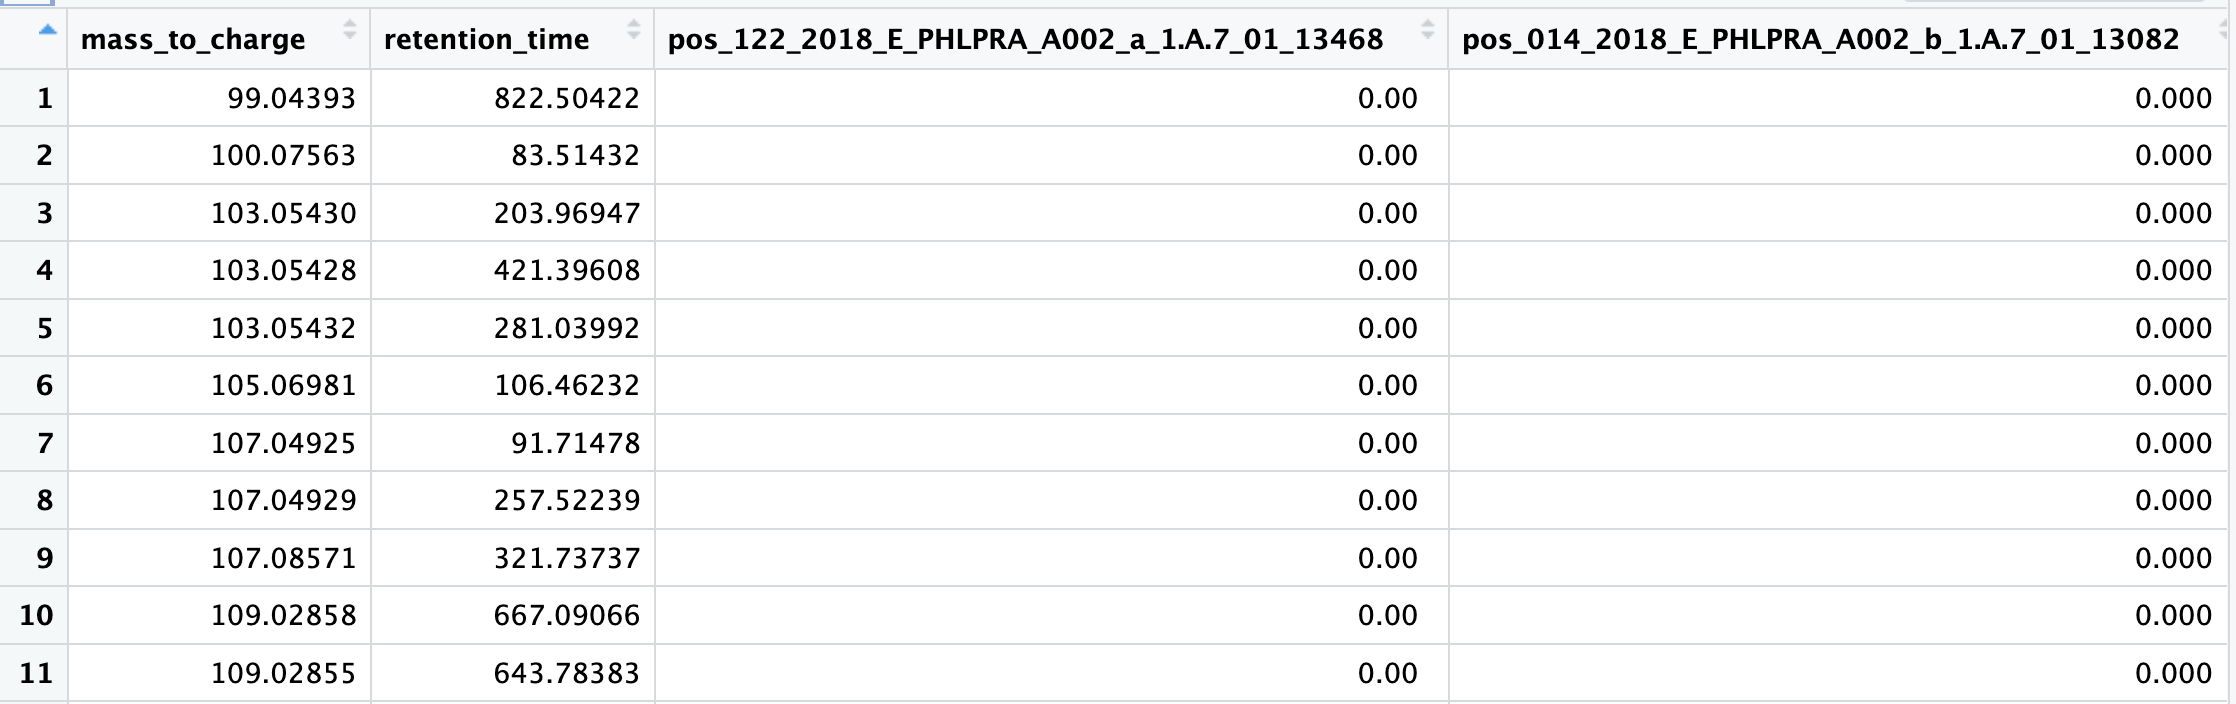
\includegraphics[width=0.9\textwidth]{images/lcms_raw.png} 
    \caption{LCMS dataset after initial processing using the \texttt{metabolighteR} package, revealing the selected columns relevant for downstream analysis.}
    \label{fig:lcms_raw}
\end{figure}

The diversity of the metabolic profile analyzed in Liquid Chromatography-Mass Spectrometry (LC-MS) makes it one of the essential tools in plant metabolomics. LC-MS has a great number of uses within the field of plant biology for plant metabolite identification and analysis. Unlike other techniques such as gas chromatography coupled to mass spectrometry, 
the steps involving derivatization are avoided in LC-MS [43]. This makes LC-MS particularly fit for the detection of varied classes, including semi-polar compounds and secondary metabolites common in plants [43]. The flexibility of LC-MS in gradient elution further allows effective separation of complex mixtures. Using different polarities of solvents 
during the elution process allows for the separation of polar and nonpolar compounds. Reverse-phase LC-MS, a widely used approach, often employs a gradient starting with an aqueous solvent and progressively increasing the proportion of an organic solvent, ensuring the efficient separation of a broad spectrum of metabolites [43]. \\


\section{R Programming}
R is an open-source and free software developed by professors Robert Gentleman from the University of Waterloo and Ross Ihaka from University of Auckland as a programming language to teach statistics [37]. This free programming language 
is widely used for statistical analysis, data visualization and graphical output [38]. Quoting the words of Ross Ihaka, “R is a computer language and run-time environment which can be used to carry out statistical (or other quantitative) computations” [37]. 
The name “R” itself comes from the shared first letters of both authors and being the successor of “S” language [37]. The strength of R is its extensive add-on packages which helps to analyse and visualize complex data. Even though R primarily has a command 
line interface, multiple third party graphical user interfaces such as Rstudio, Jupyter are available for better user friendly experience [37,38]. R is a versatile software suited for data manipulation, computational and graphical representation [39]. The GNU General 
Public License of R offers users significant freedom, including the ability to use, modify and distribute the software making it a favourite programming language for researchers across all the fields [37,39]. \\

R is often associated with statistics creating a versatile environment that incorporates many traditional and modern statistical techniques [39]. Some of these techniques are part of base R setup while others are available through additional packages. R offers a greater flexibility and control over analytical 
processes by step-by-step analysis with intermediate results saved as objects. This allows users to interact with and refine results using additional R functions [39].
R is an expression-based programming language with a straightforward syntax. It is also case-sensitive, meaning variables like “A” and “a” are distinct and names must start with a letter or a period not followed by a digit [39]. The commands in R can either be expressions or assignments. 
Expressions are evaluated, displayed and then discarded. Assignments, on the other hand, evaluate expressions and assign their results to variables without displaying it, allowing more flexible programming [39]. \\

Initially, R gained popularity for its syntax, closely resembling the S programming language, which made it easy for the S-PLUS users to transition to R. The versatility of R made it popular since it could run on various platforms, such as tablets and smartphones due to its open-source nature [8]. 
The frequent updates, including annual major release and timely bug fixes, underline the active development in R. Its advanced graphical capabilities is another very good quality among many, supporting detailed and publication-quality visuals with help of packages such as “ggplot2” surpass many competitors [8].
These visualization packages allows high-dimensional visualizations and are more user friendly [8]. R remains true to its original philosophy, offering an interactive and programmable environment for creating tools. Its strong community contributes a wide range of packages, share knowledge and support on the 
forums like Stack Overflow, allowing innovation and collaboration among users worldwide [8]. The main R system can be downloaded from the Comprehensive R Archive Network (CRAN), which also hosts many additional packages that extend R’s capabilities [8]. The R system is divided into two parts \\

\begin{itemize}
    \item The core R system, which can be downloaded from CRAN for different platforms like Linux, Windows and MacOS.
    \item Additional functionality through different packages.
\end{itemize}

R is a powerful tool for statistical computing, this along with high quality visualization capabilities provides a robust environment for machine learning (ML) and deep learning (DL) [42,8]. The availability of a wide range of supporting packages and libraries makes R a powerful tool for both traditional ML methods and modern DL techniques [42]. There are various packages available to perform ML and DL in R, some of them include caret, randomForest, keras and tensorflow. These packages contain the algorithm for different  ML and DL models. This project involves the implementation of various ML and DL models using the R programming language. \\

\section{Machine Learning}

Machine learning (ML) as the name indicates is the field of computer science which applies mathematical models and algorithms to enable the system to learn and make predictions without being programmed explicitly [18,19]. In contrast to classical programming where someone explicitly programmes an algorithm to execute predefined tasks,
ML uses a subset of (training) data to learn patterns and relationships within the data to create an algorithm which can generalize to unseen data[18]. This versatility and flexibility enables ML methods to improve performance over time, leading to advanced data driven decision making [23,18]. As a subgroup of Artificial intelligence (AI)
is often simply represented as a 3 layer model which includes an inputlayer that receives the data, a hidden second layer which processes the data according to the mathematical backend of the model and finally the third output layer that outputs the prediction [21]. The hidden layer which does the linear regression or classification differs 
according to the ML model in use and these are often compared to a single human neuron, where dendrite represents input layer, cell body corresponds to hidden layer, and axon functions as output layer [21]. ML employs four primary learning methods namely, supervised, unsupervised, semi-supervised and reinforcement learning [18]. \\

\paragraph{\textcolor{darkblue}{Supervised Learning}} 
Supervised learning is a ML approach that aims to predict a known output  based on the input data. It excels in tasks where the patterns in data can augment human decision making [18]. 
For instance, handwriting recognition or object classification (example, distinguishing an elephant and tiger). These tasks are easily done by humans and supervised learning strives to replicate 
or enhance this performance [18]. Another example would be in medicine where supervised ML identifies patterns in the electrocardiogram (ECG) which is an easy job for a trained cardiologist. 
These classification tasks from supervised learning are achieved through training an algorithm on labeled datasets containing ECG features (heart rate, rhythm and waveform shape) and their corresponding diagnosis. 
By mapping these features (X) to diagnostic outcomes (Y), the algorithm learns the function f(X) to accurately predict for new unseen ECG data [18,24]. Another common application of supervised learning is in regression and classification tasks [18]. 
Regression focuses on predicting continues numerical values such as LC-MS values from NIRS data and test scores. In contrast, classification predicts which category does the given instance belong such as elephant or tiger as seen in the previous example [23,24]. \\

\paragraph{\textcolor{darkblue}{Unsupervised Learning}} 
Unsupervised learning is considered to be more challenging compared to supervised learning since the former focuses on discovering patterns or groupings within data without predefined targets [18]. Common unsupervised learning tasks include clustering, association and anomaly detection, where the algorithm independently identifies underlying structures in the data [23,18].
For instance, clustering data points into separate groups based on the shared features (\ref{fig:ml}). 

\begin{figure}[h]
    \centering
    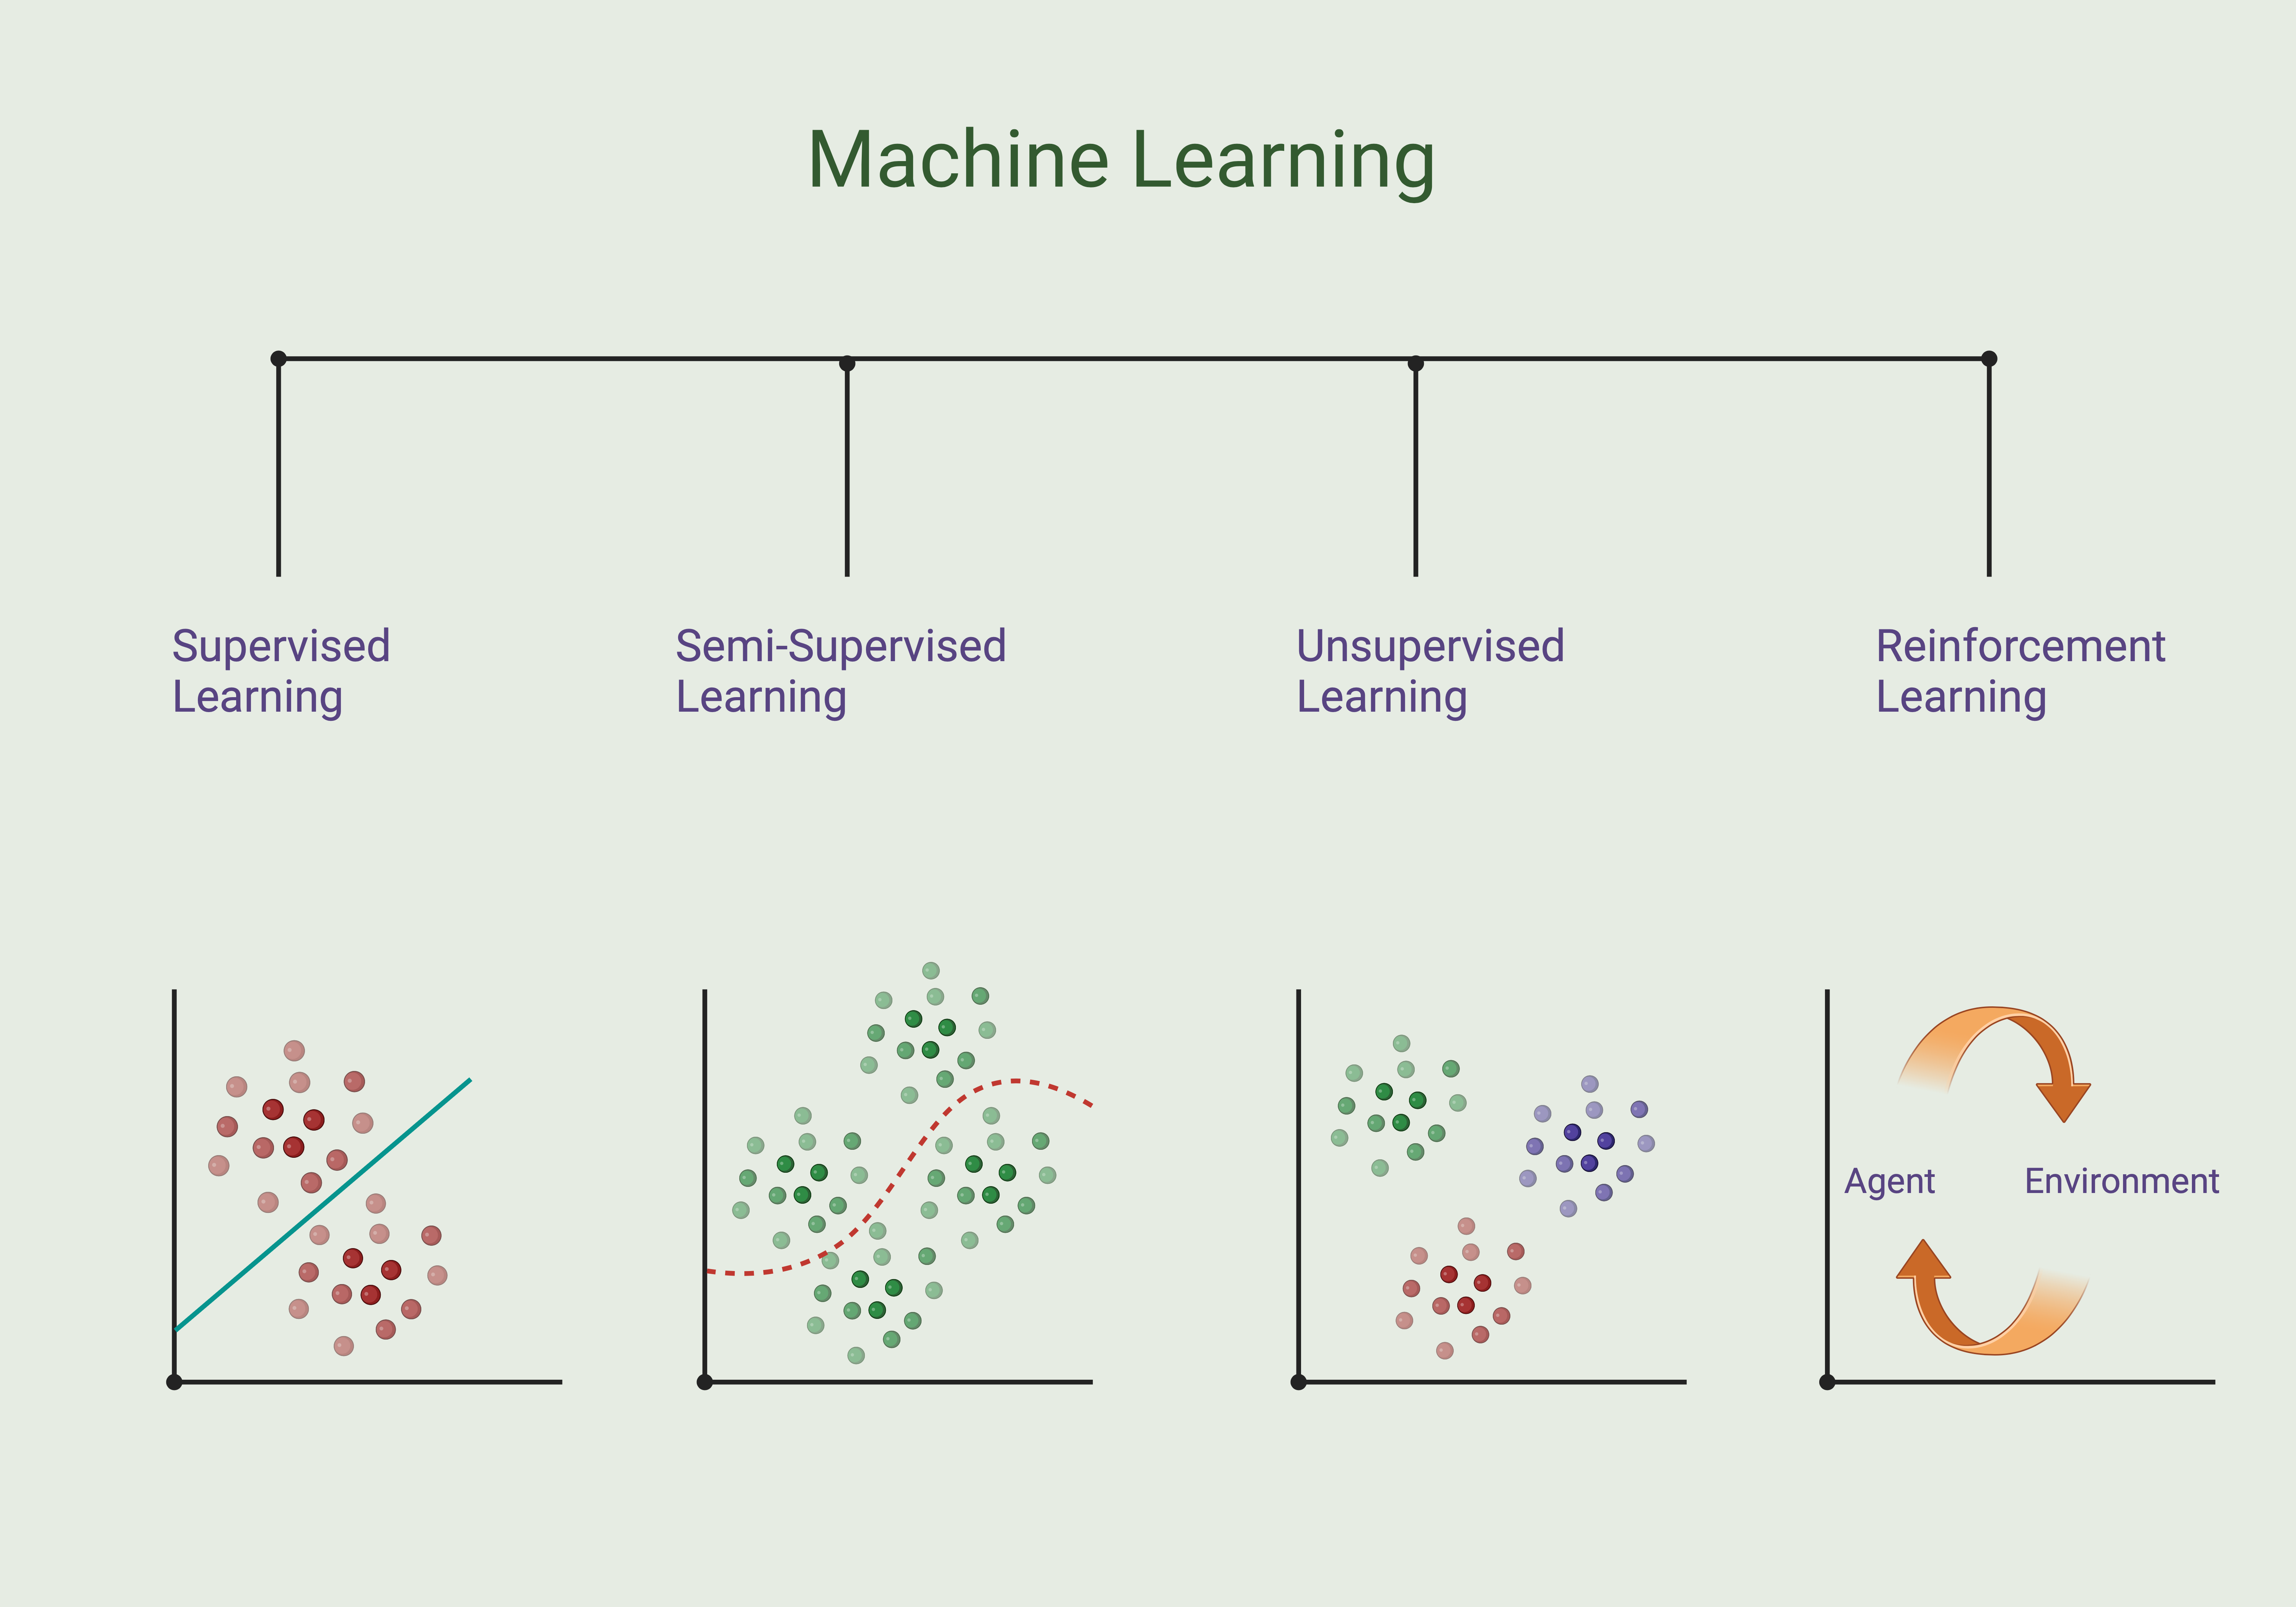
\includegraphics[width=0.6\textwidth]{images/ml.png} 
    \caption{Different machine learning models illustrating the four primary learning methods: supervised, unsupervised, semi-supervised, and reinforcement learning.}
    \label{fig:ml}
\end{figure}

\paragraph{\textcolor{darkblue}{Semi-supervised and Reinforcement Learning}}
Semi-supervised learning bridges the gap between supervised and unsupervised learning by utilizing datasets that have both labelled and unlabelled data. On the other hand, reinforcement learning mimics the human learning process, where it relies on trial and error then solely on data [24]. \\

In the era of modern molecular plant breeding, integration of ML with the large, noisy and heterogeneous data is important to uncover complex patterns and enable accurate predictions of plant features [23]. The “big data” resulting from high throughput techniques in plant sciences can be leveraged 
to drive discoveries, enhanced precision and accelerate advancement in plant research [23]. A plant genetic makeup (genotype) has a significant influence in its growth, development and biochemical composition. This results in the expression of plant traits such as yield, stress tolerance and pest resistance. 
Understanding how genotype and environment influences on phenotypes is crucial for insights into regulatory mechanisms, and development of plants [23]. This knowledge enables the  prediction of yield and other plant traits based on the genotypes under different environmental conditions, which in turn paves the 
way for modern molecular plant breeding [23]. Different ML approaches such as Partial Least Square Regression (PLSR), Random Forest (RF) and Convolutional Neural Networks (CNN)  can be employed to make predictions by leveraging patterns in the data. \\

\subsection{Partial Least Square Regression (PLSR)}
In machine learning, Partial Least Square Regression (PLSR) is a statistical method which combines the benefits of Principal Component Analysis (PCA) and linear regression to predict the outcomes [26]. It is a linear regression model which is arguably the simplest machine learning algorithm that uses a straight line to solve a regression problem [18]. PLSR uses the advantage of PCA for dimensionality reduction and the regression for prediction [27].
This fitting of linear regression between two data matrices has a wide range of application in plant biology, especially in crop breeding, ecosystem monitoring and predicting plant traits from its spectral data [25]. In PLSR, the predictor variable (often denoted as X) refers to a set of independent 
variables or features that are used to predict response variable (y). The predictor variables are typically high dimensional and often include multiple correlated features. The response variable (y) represents the outcome or dependent variable. PLSR works by identifying the latent variables, which 
summarizes the covariance between predictor and response variables. This latent variable captures the most relevant information from the predictors (X) in relation to response (y) variables, allowing the model to predict y more effectively [25,27,28]. \\

\begin{figure}[h]
    \centering
    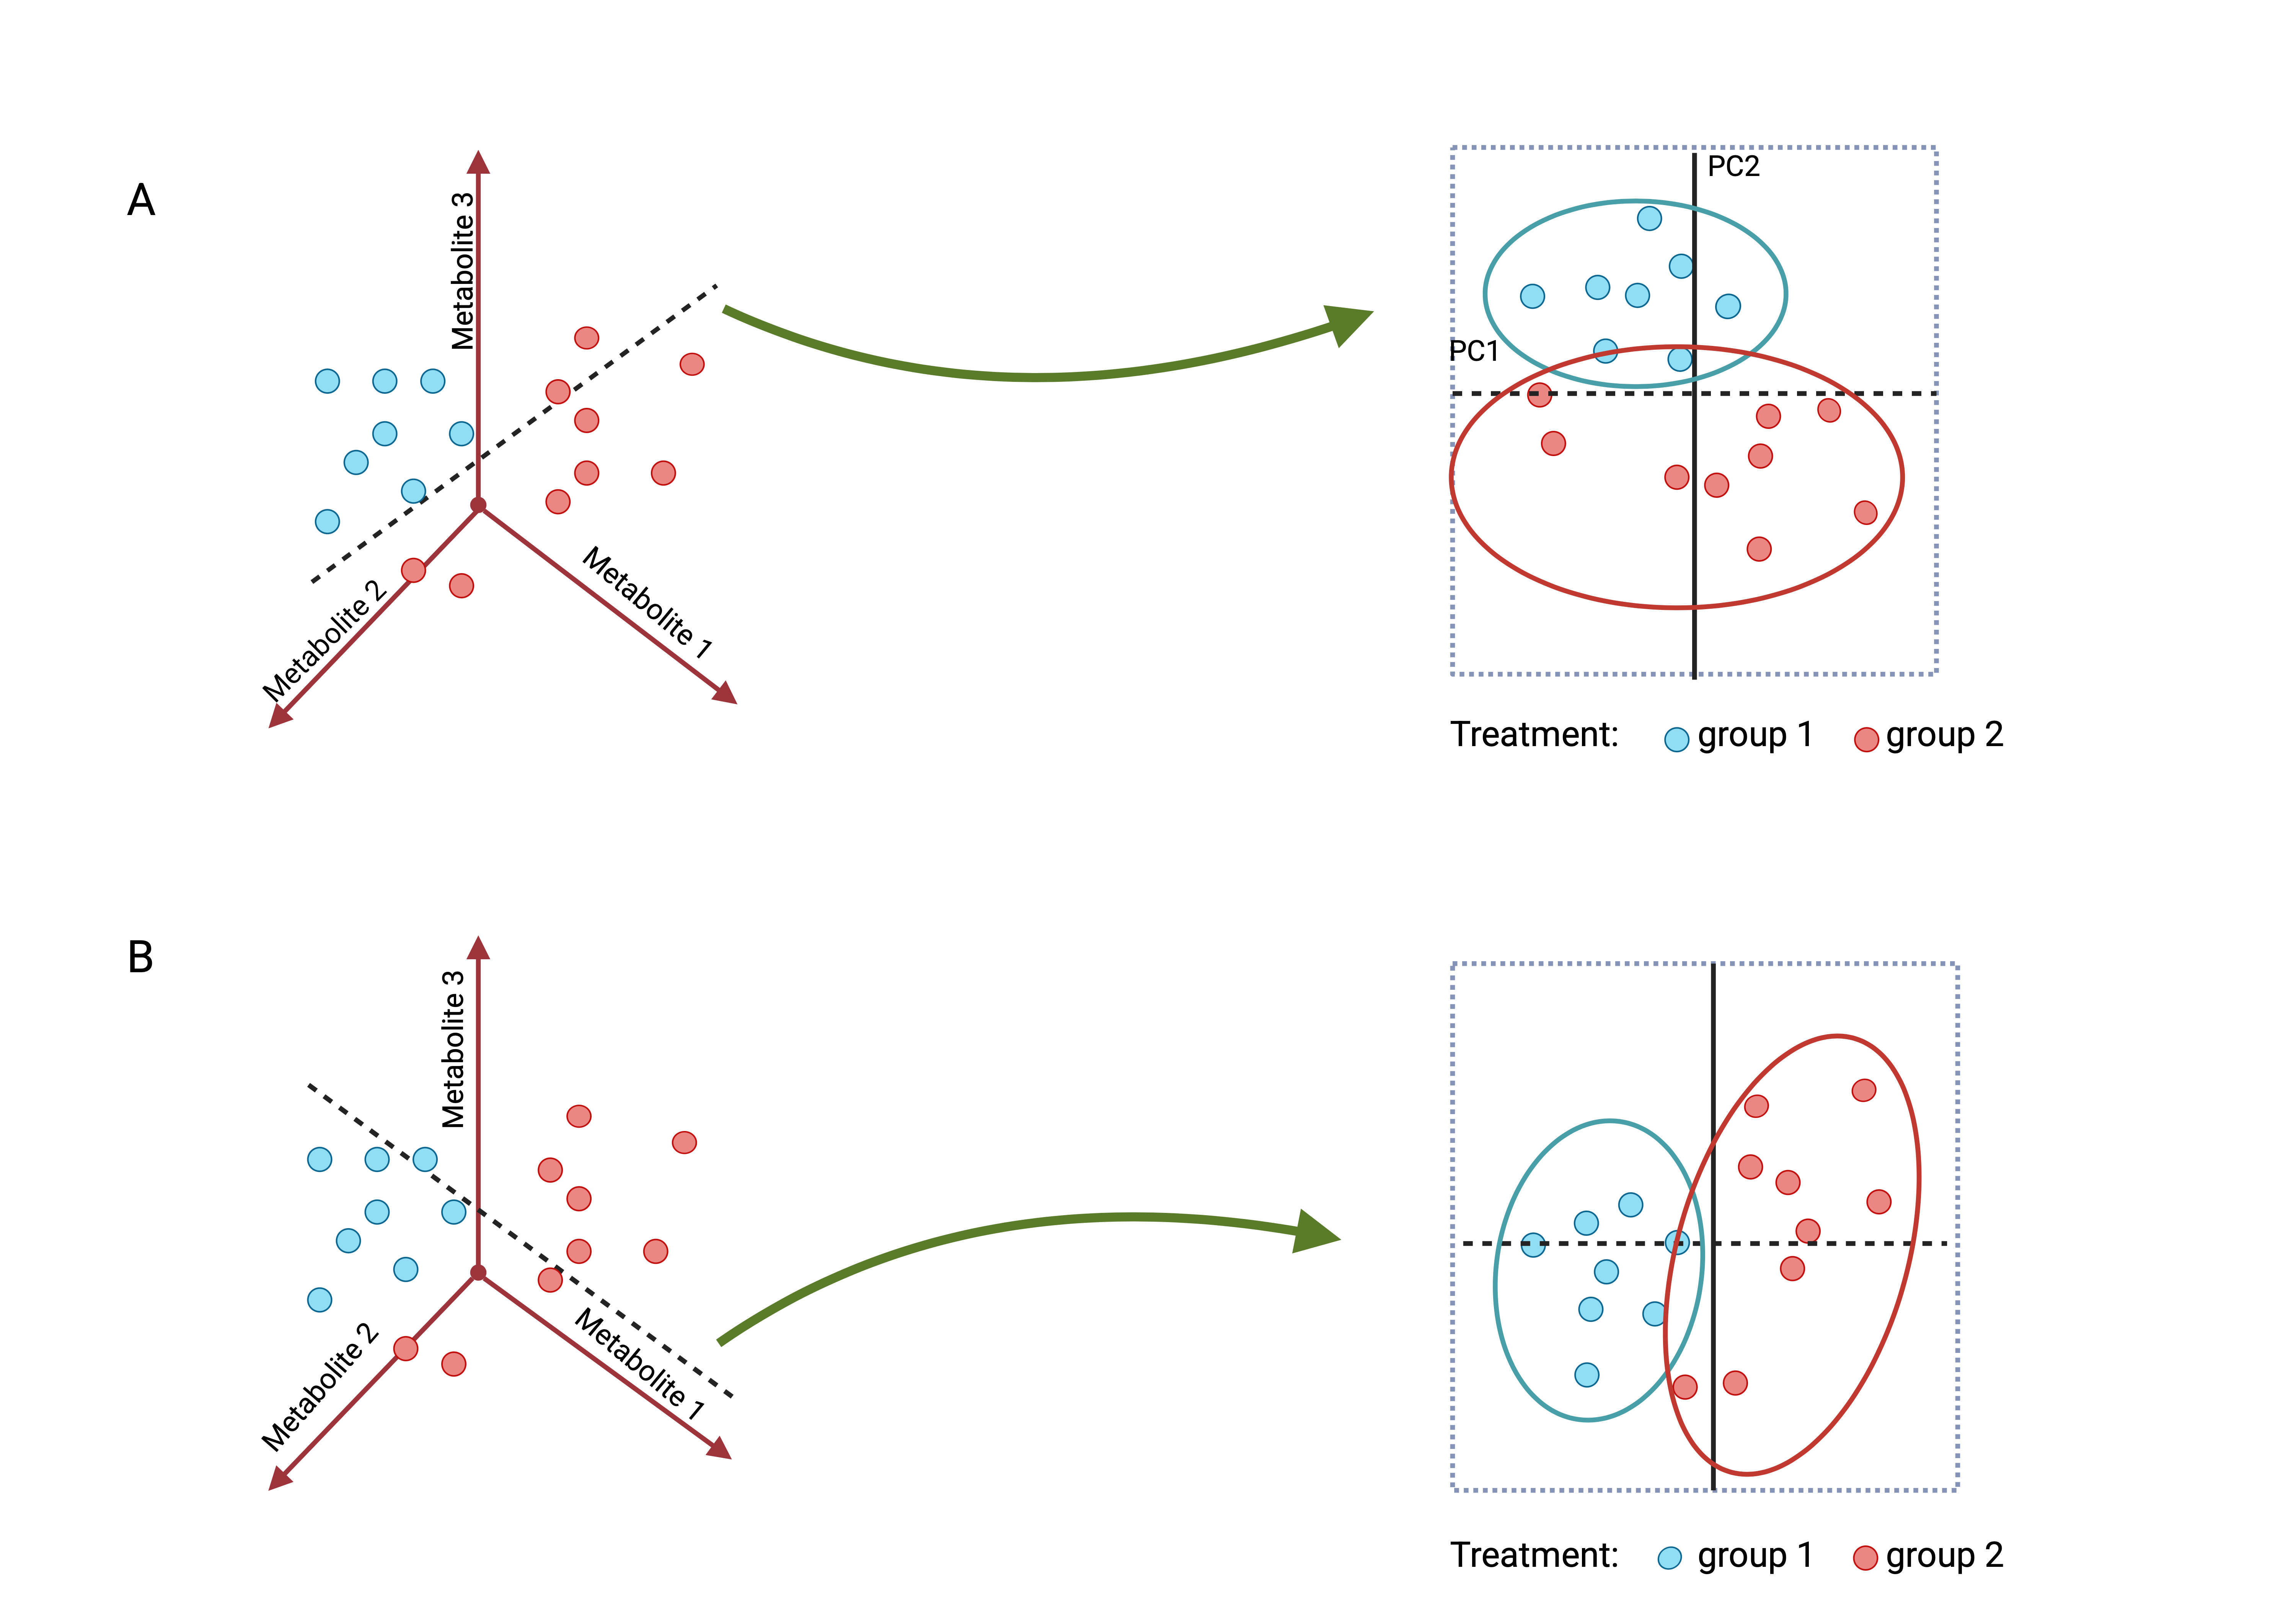
\includegraphics[width=0.6\textwidth]{images/PLSR.png}
    \caption{A comparison of PCA (A) and PLS (B). In the PCA plot, the x-axis represents a combination of variables (e.g., three metabolites) that captures the greatest variation in the dataset, independent of group classification. In contrast, PLS focuses on explaining the relationship with an explanatory variable, such as "Treatment" in this example}
    \label{fig:plsr}
\end{figure}

Principal Component Analysis (PCA) uses the principal components as explanatory variables to capture most of the variance in predictor variables (X), ensuring dimensionality reduction while retaining most of the data’s variability. 
Partial Least Squares (PLS) prioritize relevance to both X (predictor) and y (response) variables, rather than maximising the variance in X alone (\ref{fig:plsr}) [27]. By combining the PCA with linear regression, PLSR constructs 
the latent variable that summarizes predictor variables and maximises their relevance to the response variables. This makes PLSR particularly suitable for high dimensional datasets such as spectral data from NIRS instruments. \\

\subsection{Random Forest (RF)}
Random Forest (RF) is a non-linear ensemble technique used in machine learning which is also depicted as a forest of decision trees [18][29]. Random forest is commonly used for classification tasks, though it can also be 
applied to regression such as predicting the leaf trait values from the NIRS data [18]. It is a supervised learning method consisting of decision trees and the root node serves as the initial point for dividing the dataset. 
Recursive partition in which the data is separated into two binary part begins with the root node [18]. RF combines multiple trees to improve accuracy, robustness and reduce overfitting [18,29].
In the classic tree based model, the dataset is divided into two groups based on the certain criteria until it encounters a predetermined stopping condition. The endpoints of a decision tree, known as leaf nodes, 
represents the final data division. A random forest model consisting of an ensemble of decision trees, can be utilized for both regression and classification tasks, depending on the partitioning strategy and stopping criteria [30]. 
RF has proven its importance in many scientific domains and one of which was in environmental science, in a study employed learning algorithms such as Least Absolute Shrinkage and Selection Operator (LASSO) Regression, RF and neural network to 
predict ragweed pollen concentrations, with RF delivering the most accurate predictions [30,31]. A graphical representation of the RF model with decision trees can be found in the figure (\ref{fig:rf}) . \\

\begin{figure}[h]
    \centering
    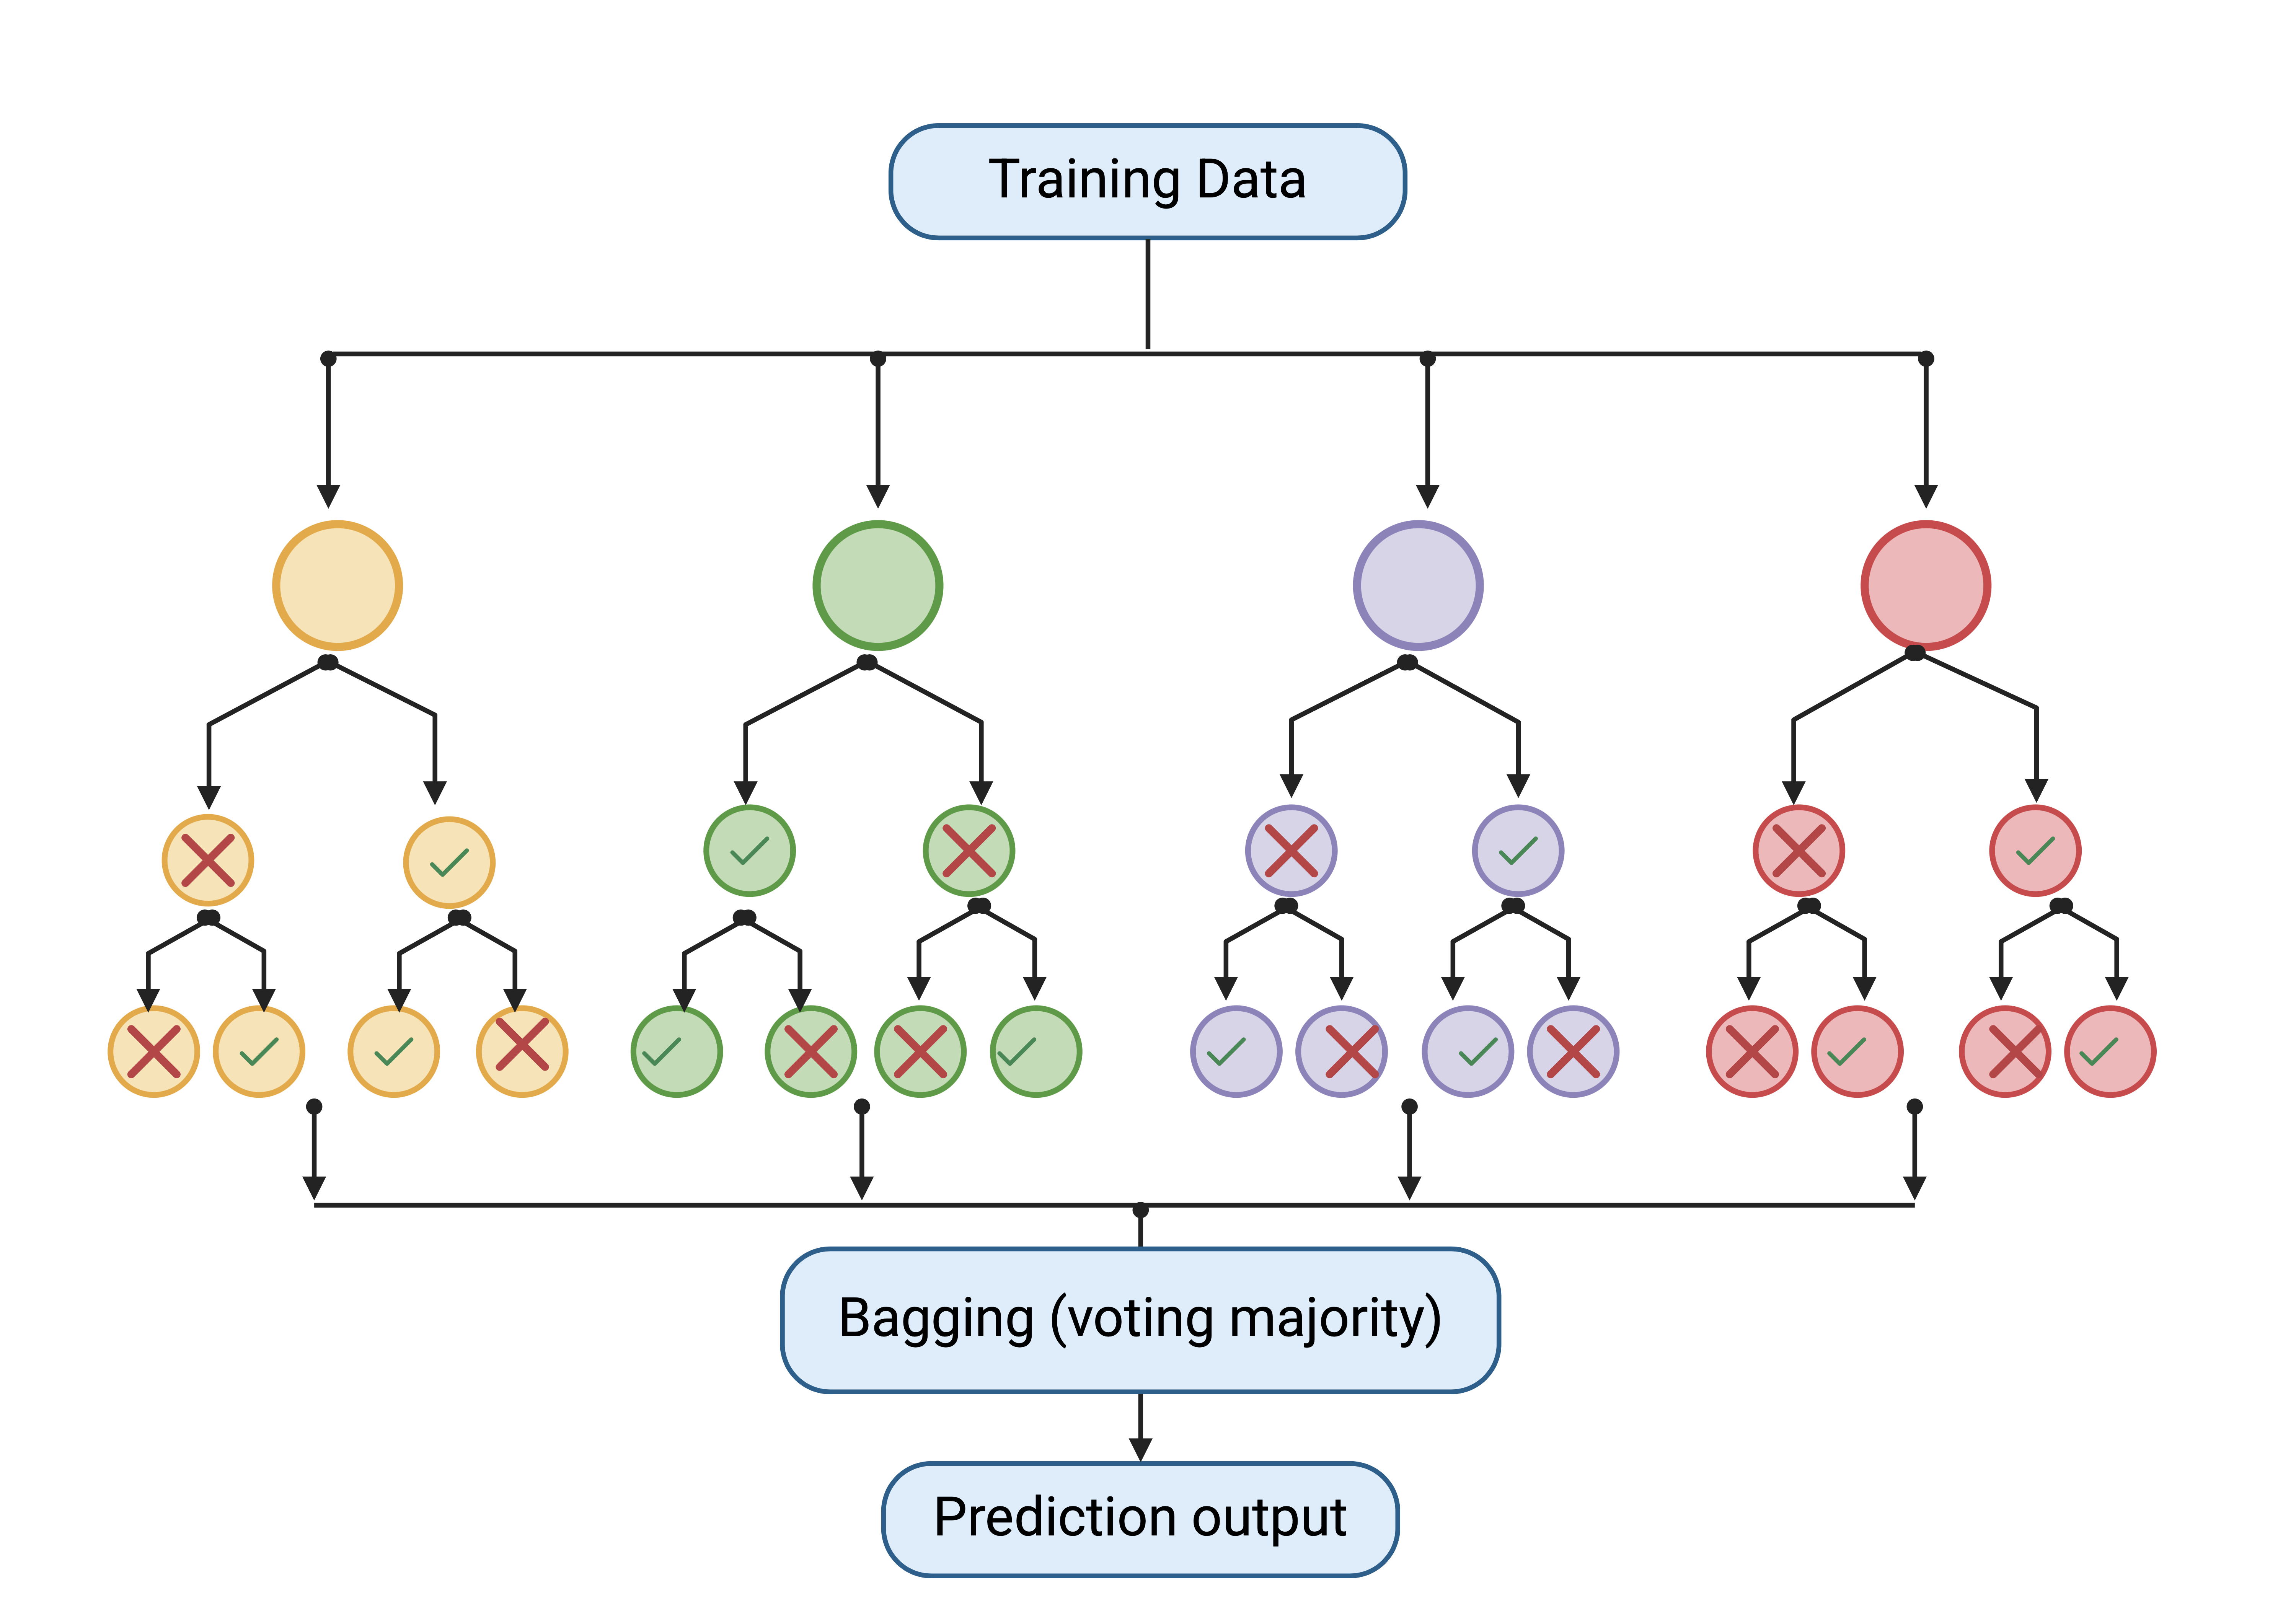
\includegraphics[width=0.6\textwidth]{images/rf.png}
    \caption{Schematic representation of a Random Forest model (classification).}
    \label{fig:rf}
\end{figure}

Random Forest often outperforms linear regression models since, linear regression assumes a linear relationship between the variables. Even though this makes linear regression easier to interpret, it limits their flexibility in capturing complex patterns in the dataset. 
On the flip side, RF can easily adapt to non linear relationships, making them better flexible and suited for such tasks [30]. The RF algorithm estimates the error rate by out-of-bag (OOB) during training time. Each tree in the model is built using a subset of data, called a 
bootstrap sample and about one third of the data is left out during this process. These excluded data points are the OOB. Hence, minimizing the OOB is crucial for better model performance and robustness [30]. \\

\textbf{Mathematical Explanation of Random Forest Regression} \\
For regression tasks, the random forest works differently compared to classification but the core principles remain the same. The terminal node of RF in regression takes the average of predictions from the individual trees [44]

\begin{itemize}
    \item \textbf{Bootstrapping and Tree Construction} \\
    Each tree in a RF model is trained using a bootstrap sample, which is a subset of the sample from the training data of the original dataset. Approximately one third of the samples (data points) are left out during bootstrap sampling for each tree and these left out samples are referred to as Out-Of-Bag (OOB) samples.
    Given a dataset \( D = \{ (x_1, y_1), (x_2, y_2), \dots, (x_n, y_n) \} \), where:
    \begin{itemize}
        \item \( x_i \) represents the feature (e.g., spectral data),
        \item \( y_i \) represents the response variable (e.g., SLA, LDMC, or other traits),
    \end{itemize}
    For each tree (\( t \)), a bootstrap sample \( D_t \) is taken out of dataset \( D \), and the OOB for that tree is calculated as:
    
    \[D_t^{\text{OOB}} = D \mathbin{-} D_t

    
    \item \textbf{Model training and Prediction} \\
    Each tree in a RF model is trained with a separate bootstrap sample (\( D_t \)) and later exposed to test data for predictions to be made.
    For the test data \( X_{\text{test}} \), the prediction from each tree (\( t \)) is denoted as \( \hat{y}_t(x_{\text{test}}) \). The final prediction from the RF is obtained by taking the average value of predictions from all the individual trees:
    \[\hat{y}_{\text{RF}}(x_{\text{test}}) = \frac{1}{T} \sum_{t=1}^{T} \hat{y}_t(x_{\text{test}})
    \]
    where:
    \begin{itemize}
        \item \( \hat{y}_t(x_{\text{test}}) \) is the prediction from the \( t \)-th tree,
        \item \( T \) is the total number of trees in the Random Forest.
    \end{itemize}
\end{itemize}


In this project, we will be using RF models to do regression tasks on NIRS data and compare the coefficient of determination R2, RMSE and training time with that of linear model and neural network, we will also discuss developing the RF model and associated functionalities. \\



\subsection{Convolutional Neural Network (CNN)}

Convolutional Neural Network (CNN) is a type of deep learning (DL) model inspired by the way neurons in the brain process visual information [32,33]. It is primarily composed of three core components: A convolutional layer that extracts features, a pooling layer to reduce the 
dimensionality of data and a fully connected layer that produces the final output [32]. Out of these three main layers, the convolutional layer is considered as a fundamental component of a CNN, consisting of a series of mathematical operations, including convolution, which is 
a distinct form of linear regression [32]. It involves the application of kernels, which is a small array of numbers across the input (tensor) to compute elementwise products. These results are summed to create an output called feature map. Each kernel extracts a different feature 
of the input data and thereby different feature maps with different characteristics of the input data.The number of kernels determines the depth of the data and is also selected based on the scale of input data. A stride is known as the step size for moving the kernel across the tensor, 
commonly a stride of 1 is used. To capture the outermost element in the tensor, zero padding technique, which involves adding rows and columns of zero on the sides of input tensor is used to prevent downsizing in the convolutional layer [32]. After the convolutional layer the feature map 
is then processed through a nonlinear activation function and then to the pooling layer for downsampling [32]. In CNN the widely used pooling method is max pooling, which divides the feature map into small patches and then keeps only the highest values from each patch and ignores the rest. 
The output from the last pooling layer is flattened to 1 dimensional array and passed to fully connected layers, where each input is connected to every output with a learnable weight. These layers map the extracted features to the final output [32]. \\

\begin{figure}[h]
    \centering
    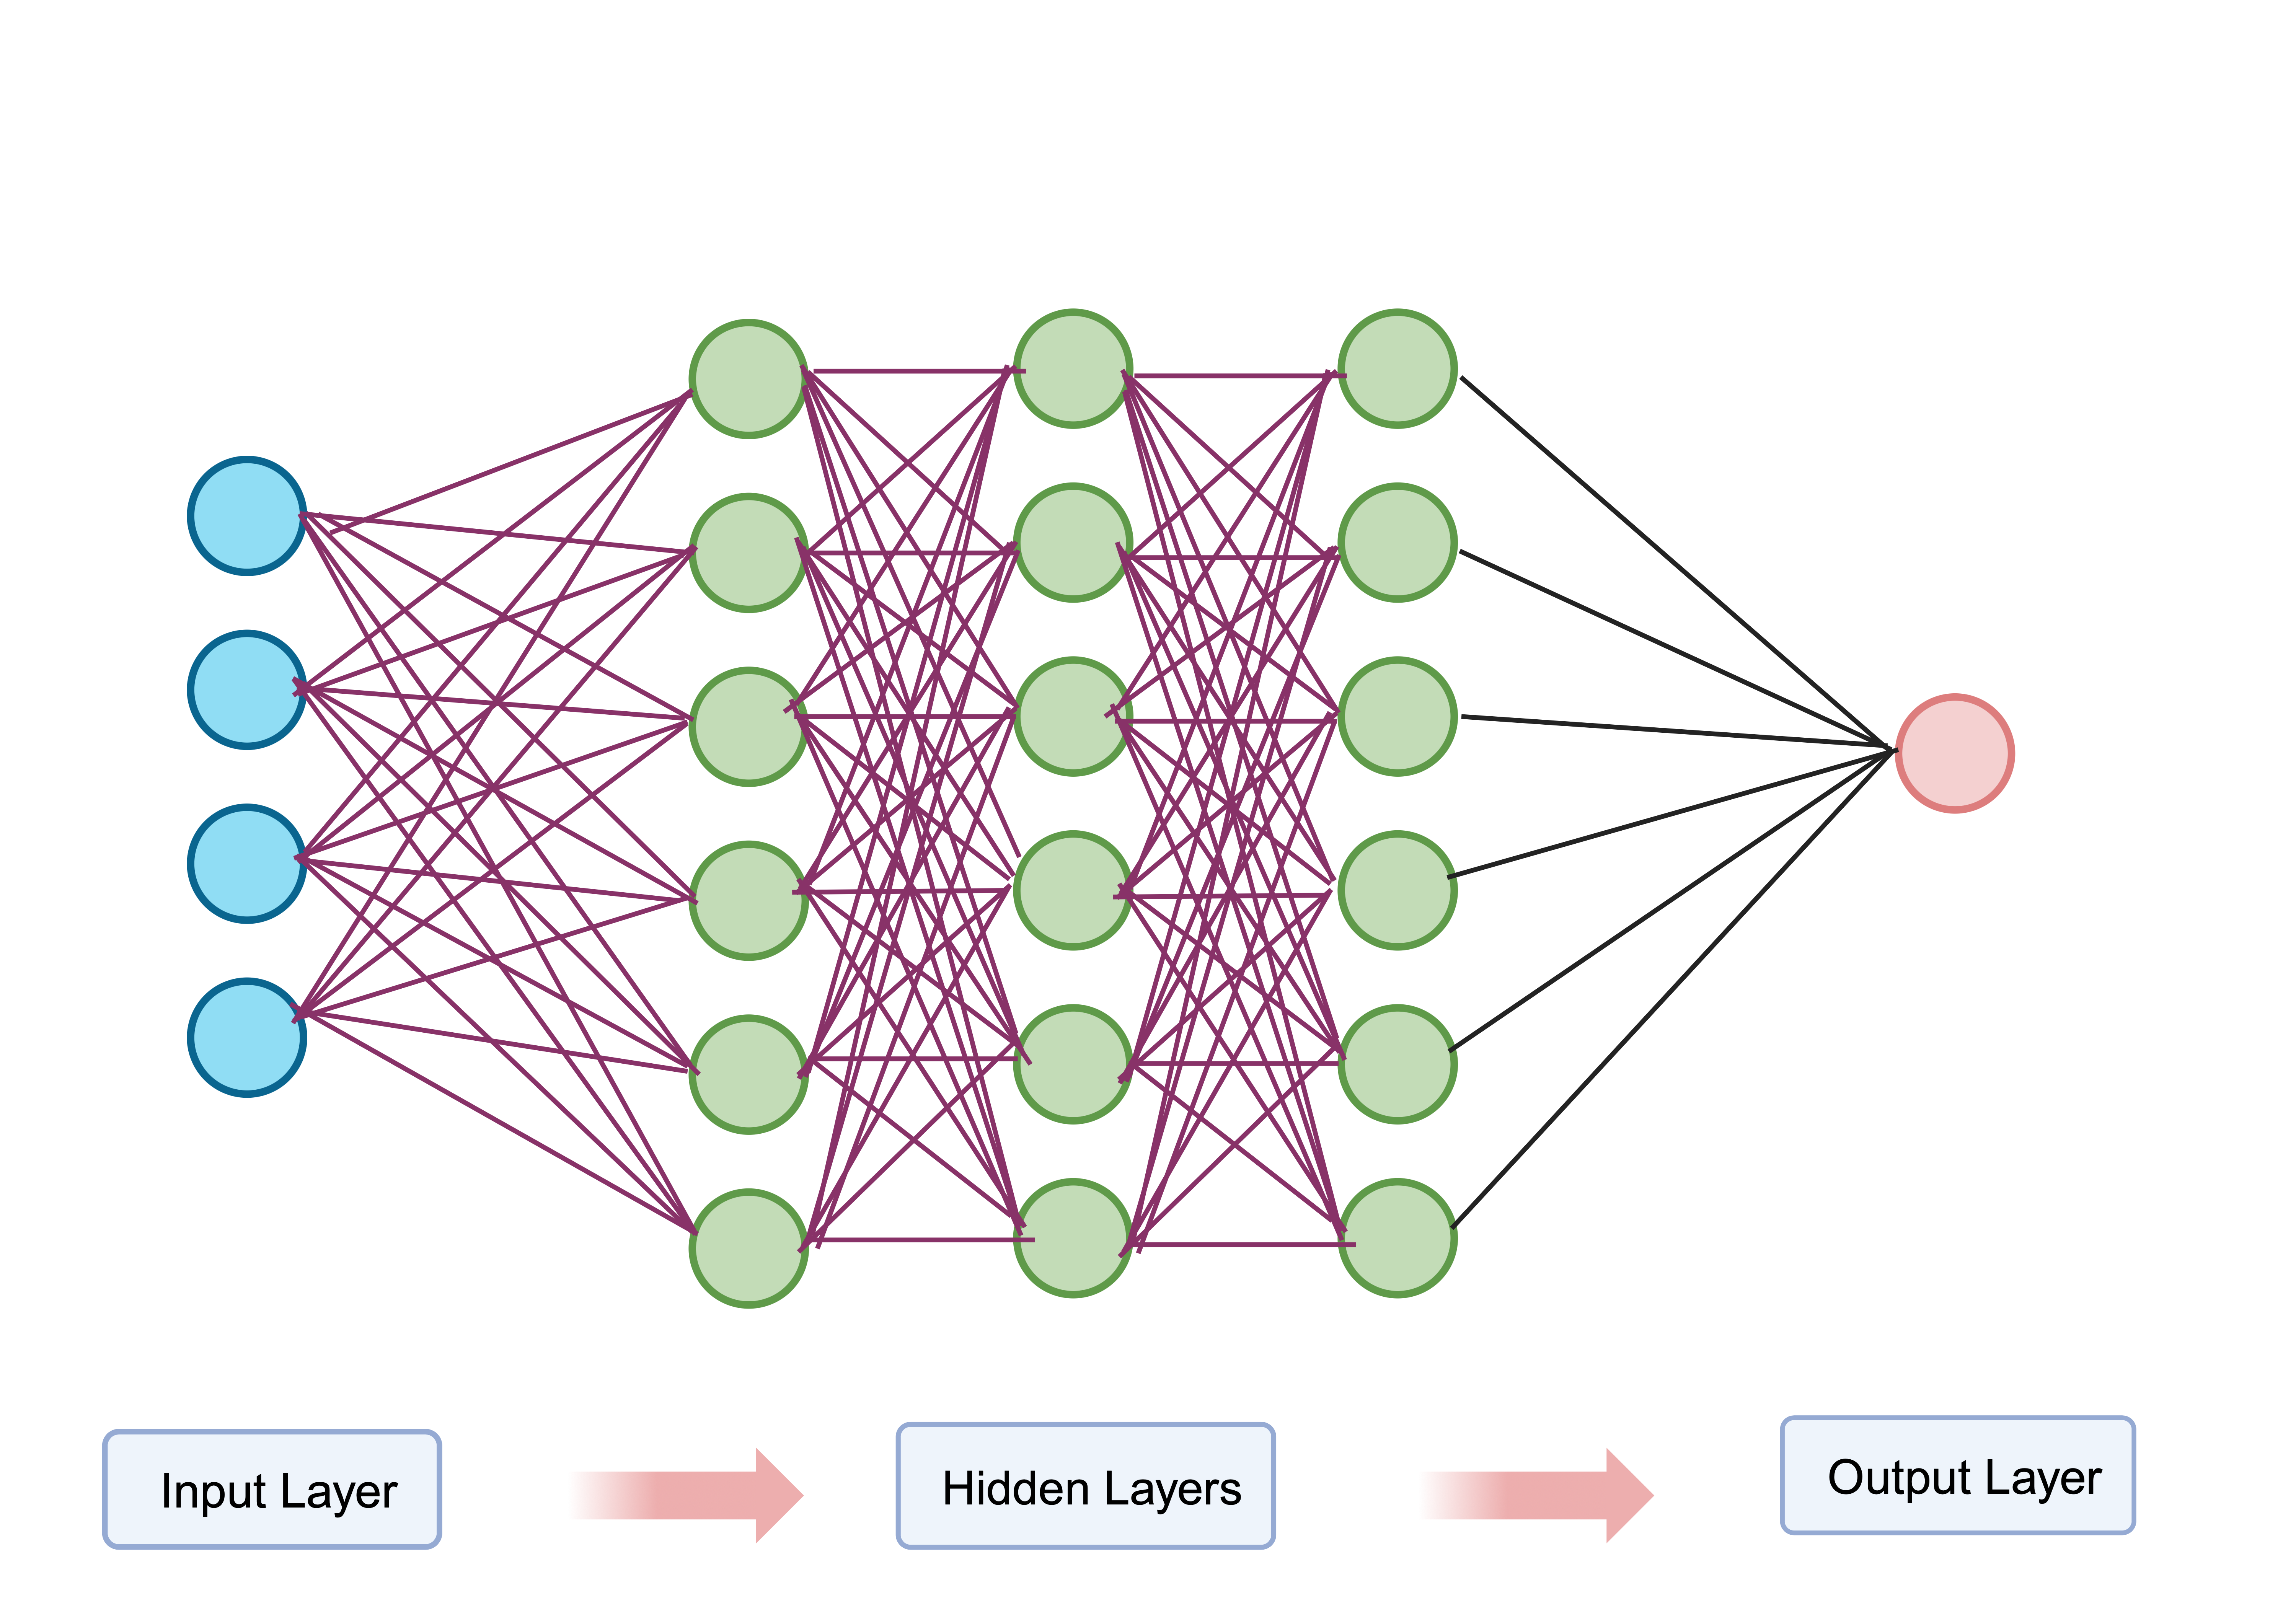
\includegraphics[width=0.6\textwidth]{Figures/cnn.png}
    \caption{Schematic representation of Convolutional Neural Network }
    \label{fig:cnn}
\end{figure}

A loss function evaluates how well the predicted values match the actual ones.  For classification cross-entropy loss is commonly used whereas mean squared error (MSE) is preferred for regression tasks. Choosing the right loss function is essential and is determined according to the given task [32]. In deep neural network training, the weights of each neuron is estimated to establish an accurate relationship between inputs and outputs with a desired level of precision [34].
It is categorized into supervised learning, for classification and regression tasks, and unsupervised learning, for clustering with input data only. Several methods are employed for training deep neural networks, including Backpropagation, Gradient Descent, Stochastic Gradient Descent (SGD), and others. Among these, SGD stands out as one of the simplest and most widely used optimization algorithms in machine learning [34]. Adaptive Moment Estimation (ADAM) is an advanced 
optimization algorithm which combines the benefits of two SGD variants: Adaptive Gradient Algorithm (AdaGrad) and Root Mean Square Propagation (RMSProp) [34]. It requires minimal memory and dynamically adjusts the learning rate for each parameter, making it more computationally efficient [34]. In this project CNN is employed to predict the output values from NIRS data. \\






%-----------------------------Implementation-----------------------------------------------------

\chapter{Implementation}
\section{R Toolbox Development}
The idea of developing of a new toolbox arise from the realization that existing R packages were lacking functions to compartmentalize spectral data in a way that could be easily integrated into the Bioconductor ecosystem. Bioconductor offers remarkable advantages in terms of integration and interoperability. These are highly valuable for advanced data analysis. 
Existing packages commonly used in ecological studies, such as \textbf{FieldSpectra}, \textbf{plantspec}, and \textbf{spectacles}, were reviewed. However, none provided functionality to convert high-dimensional spectral data into a SummarizedExperiment object, a data structure widely used in Bioconductor for organizing and analyzing complex datasets. \\

After recognizing the potential applications of the SummarizedExperiment framework in plant biology, along with its ability to simplify workflows and facilitate future analyses, a decision was made to develop a toolbox to address this gap. The primary objective during development was to make sure vendor independence, making the toolbox broadly applicable. Vendors 
such as Malvern Panalytical offer software for processing data from instruments such as the ASD FieldSpec 4, while the SVC HR-1024i from Spectra Vista Corporation requires additional computational effort to structure the data for analysis.
In addition, the ASD FieldSpec 4 generates binary output files. To process these files, functions from the \texttt{FieldSpectra} package were utilized as a foundation, with additional custom functions developed to convert the data into SummarizedExperiment objects. The entire workflow, including data reading, processing, and conversion, is detailed in this chapter.\\

\subsection{Toolbox: nearspectRa}
%\begin{wrapfigure}{r}{0.4\textwidth}
    %\centering
    %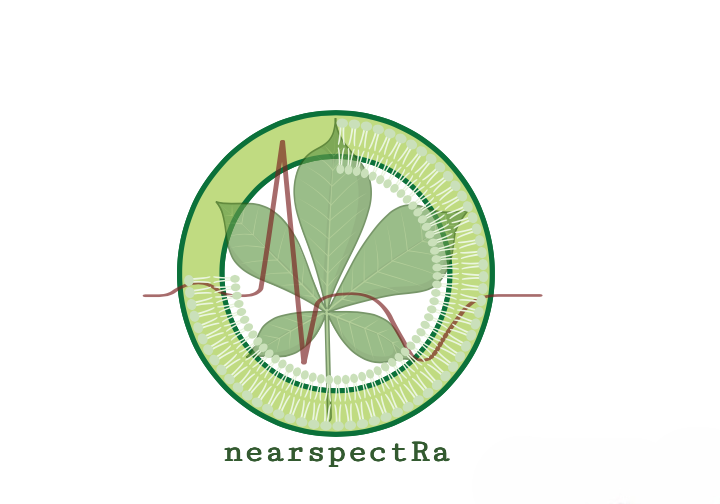
\includegraphics[width=\linewidth]{Figures/nearspectra.PNG} 
    %\caption{The official logo of the \texttt{nearspectRa} package.}
    %\label{logo }
%\end{wrapfigure}
The toolbox, named \textbf{nearspectRa}, is specifically designed to handle  Near-Infrared Spectroscopy (NIRS) data. This name was chosen to align with its functionality and field of usage, focusing on plant metabolic phenotype analysis. The toolbox is publicly available on GitHub and can be accessed at the following link: \href{https://github.com/georgejr45/nearspectRa}{GitHub Repository} \\


\subsection{Functions of nearspectRa}
\textbf{Function 1: \texttt{read\_summarizedexperiment\_asd}} \\

\textbf{Key Features:}
\begin{itemize}
    \item Input: A path to either a single .asd file or a directory containing multiple .asd files.
    \item Output: A SummarizedExperiment object with: 
    \begin{itemize}
        \item Assays: Reflectance data as a matrix where rows are wavelength and columns are samples.
        \item colData: Sample metadata.
        \item rowData: Wavelength metadata.
    \end{itemize}
    \item Dependencies: Utilizes \texttt{read.asd} and \texttt{extract.metadata} from the FieldSpectra package for reading and extracting data, and the \texttt{SummarizedExperiment} library from Bioconductor.
\end{itemize}

\textbf{Pseudocode:} 

\texttt{Function: read\_summarizedexperiment\_asd(path):} \\

\begin{tabbing}
\hspace*{2em} \textbf{Input:} \= \texttt{path} to a single \texttt{.asd} file or a directory containing multiple \texttt{.asd} files. \\
\hspace*{2em} \textbf{Output:} \= A \texttt{SummarizedExperiment} object.
\end{tabbing}



\begin{enumerate}
    \item Check if the path is a file or directory.
    \item If it is a directory, list all \texttt{.asd} files in the directory.
    \item For each \texttt{.asd} file:
    \begin{enumerate}
        \item Use \texttt{read.asd} to extract spectral data.
        \item Use \texttt{extract.metadata} to obtain sample metadata.
    \end{enumerate}
    \item Combine spectral data and metadata into matrices.
    \item Create a \texttt{SummarizedExperiment} object with:
    \begin{itemize}
        \item Assays: Spectral data matrix (rows: wavelengths, columns: samples).
        \item ColData: \texttt{DataFrame} of sample metadata.
        \item RowData: \texttt{DataFrame} of wavelength information.
    \end{itemize}
    \item Return the \texttt{SummarizedExperiment} object.
\end{enumerate}

\textbf{Example Usage:}

\begin{lstlisting}[language=R, style=mystyle]
    path <- "path/to/your/asd/files"
    se <- read_summarizedexperiment_asd(path)
    print(se)
    \end{lstlisting}

\begin{figure}[h]
    \centering
    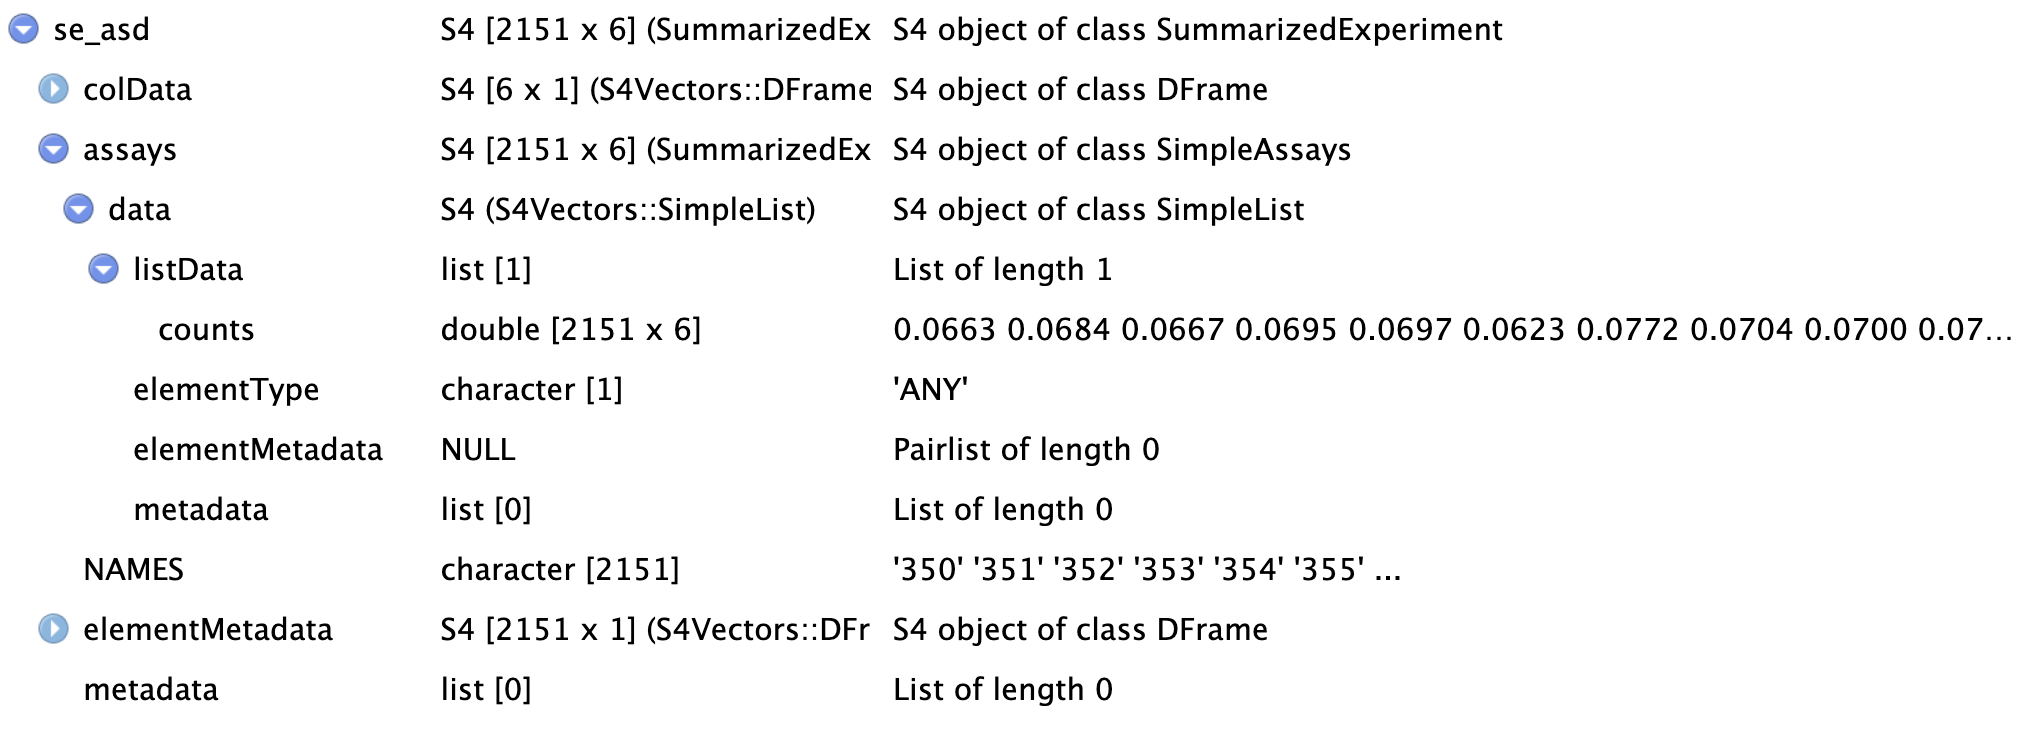
\includegraphics[width=0.6\textwidth]{Figures/se_asd_1.png}
    \caption{Example output of the \texttt{read\_summarizedexperiment\_asd function}}
    \label{Figure 2}
\end{figure}

\textbf{Function 2: \texttt{read\_summarizedexperiment\_sig}} \\

\textbf{Key Features:}
\begin{itemize}
    \item Input: A path to a single \texttt{.sig} file or a directory containing multiple \texttt{.sig} files.
    \item Output: A \texttt{SummarizedExperiment} object with:
    \begin{itemize}
        \item Assays: Reflectance data as a matrix where rows are wavelengths and columns are samples.
        \item colData: Sample metadata.
        \item rowData: Wavelength metadata.
    \end{itemize}
    \item Dependencies: Utilizes \texttt{readLines} for file reading, \texttt{grep} for pattern matching, and the \texttt{SummarizedExperiment} library from Bioconductor.
\end{itemize}

\textbf{Pseudocode:}

\texttt{Function: read\_summarizedexperiment\_sig(path):} \\

\begin{tabbing}
\hspace*{2em} \textbf{Input:} \= \texttt{path} to a single \texttt{.sig} file or a directory containing multiple \texttt{.sig} files. \\
\hspace*{2em} \textbf{Output:} \= A \texttt{SummarizedExperiment} object. \\
\end{tabbing}

\begin{enumerate}
    \item Check if the path is a file or directory.
    \item If it is a directory, list all \texttt{.sig} files in the directory.
    \item For each \texttt{.sig} file:
    \begin{enumerate}
        \item Use \texttt{readLines} to read the file content.
        \item Extract the sample name from the line starting with \texttt{name=}, or use the file name if not present.
        \item Extract spectral data starting from the line that begins with \texttt{data=}.
        \item Organize the data by wavelengths (first column) and reflectance (fourth column).
    \end{enumerate}
    \item Combine all data frames by wavelengths, filling missing values with \texttt{NA}.
    \item Create a \texttt{SummarizedExperiment} object with:
    \begin{itemize}
        \item Assays: Reflectance data matrix (rows: wavelengths, columns: samples).
        \item colData: \texttt{DataFrame} containing sample names.
        \item rowData: \texttt{DataFrame} containing wavelengths.
    \end{itemize}
    \item Return the \texttt{SummarizedExperiment} object.
\end{enumerate}

\textbf{Example Usage:}

\begin{lstlisting}[language=R, style=mystyle]
    path <- "/path/to/sig/files"
    se <- read_summarizedexperiment_sig(path)
    print(se)
\end{lstlisting}

\begin{figure}[h]
    \centering
    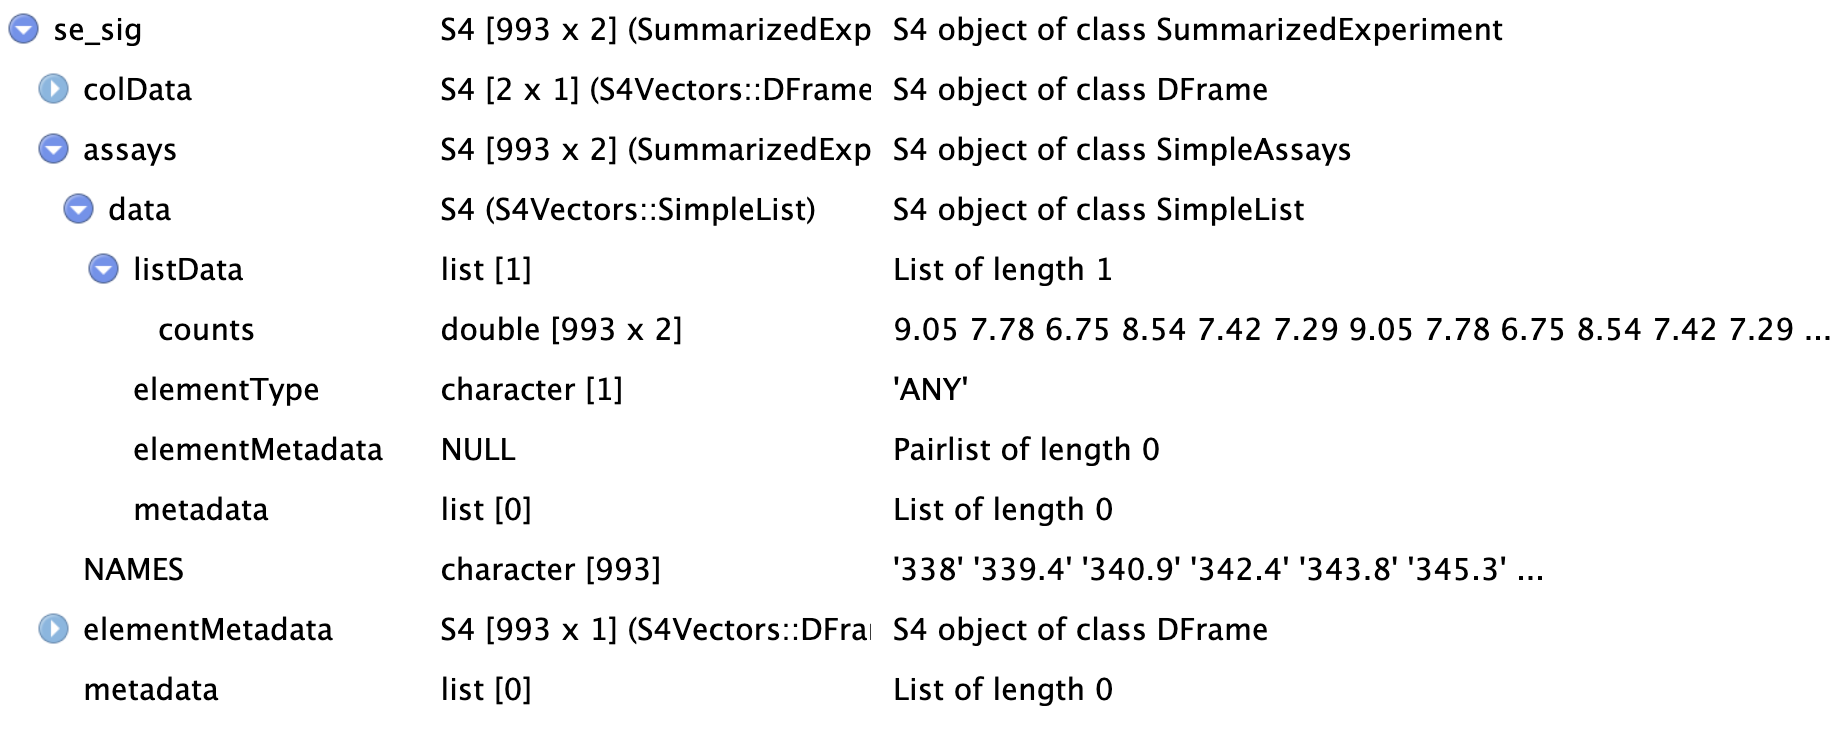
\includegraphics[width=0.6\textwidth]{Figures/se_sig.png}
    \caption{Example output of the \texttt{read\_summarizedexperiment\_sig function}}
    \label{Figure 2}
\end{figure}

\subsection{Package Development Overview}
\subsubsection*{Purpose and Objectives}
This package is aim to ease the NIRS data processing by reading the raw data and outputs a \texttt{SummarizEdexperiment} object. The programming language and tools used for this development process is mentioned below. \\

\subsubsection*{Language}
\textbf{R}: is the core programming language used for the development. It is choosen because of its powerful data analytical capabilities and wide usage in bioinformatics. The R version 4.4.0 ( eleased on April 24, 2024 ) has been used for this project.

\subsubsection*{Libraries and Dependencies}
Base R Functions: These functions come pre-installed and do not require additional libraries or packages. For instance, readLines, list.files, files.info \\
\texttt{\href{https://github.com/serbinsh/R-FieldSpectra}{FieldSpectra}}: is Used for reading the ".asd" files and to extract the metadata. The version used is FieldSpectra $0.9.7$\\
\texttt{\href{https://github.com/Bioconductor/SummarizedExperiment}{SummarizedExperiment}}: is central to this package and it enable structured storage of spectral data and integrate to the bioconductor world. The version used is $1.34.0$ \\
\texttt{\href{https://github.com/r-lib/roxygen2}{roxygen2}}: is used for generating documentation directly from inline comments. The version used is $7.3.2$ 

\subsubsection*{Version Control} 
One of the main challenges during software development is tracking and documenting the code during the development process. These challenges include, managing multiple script versions or integrating collaborator edits. Manuel merging and making multiple copies of each version is time consuming and error-prone [46].To overcome this challenge, Git is used for version control and collaborative development. A git version of $2.32.0$ is used.\\

\textbf{Examples of few git commands used in this project are given below:}
\begin{lstlisting}[language=bash, style=mystyle]
# Navigate to the project directory
cd/path/to/the/project

# Initialize a Git repository
git init

# Add a remote repository
git remote add origin https://github.com/username/project.git

# Check the status of the repository
git status

# Stage all files for commit
git add .

# Commit the changes with a message
git commit -m "First commit"

# Push the changes to the remote repository
git branch -M main  # Rename branch to main
git push -u origin main
\end{lstlisting}


\subsubsection*{Testing and Validation} 
Unit tests are implemented under \textit{test} directory to ensure a robust function performance across different datasets. \texttt{testthat} package is used for the unit test development.

\subsubsection*{Documentation} 
Documentation is a fundamental aspect of software development, regardless of the programming language or platform. It serves as a vital tool for communication between developers and end users, providing the necessary information for effectively utilizing the software to its full potential [45]. In developing \texttt{nearspectRa}, we prioritized clear and comprehensive documentation to ensure the package is user-friendly, while adhering to FAIR principles—Findable, Accessible, Interoperable, and Reusable. This documentation was created with the help of the \texttt{roxygen2} package version $7.3.2$.

\subsection{Usage and Integration}
 
........................................................

\subsection{Challenges and Future Work}
This package can be further developed to accommodate more functions and fine tune to make it suit for other analytical data as well. Future work can also include the integration of Artificial Intelligence to address the growing challenges in data analysis. 


\section{Contributions elsewhere}
\subsection{GitHub Actions to R-FieldSpectra}

During the development of nearspectRa for processing NIRS data, we identified an opportunity to enhance the widely used R-FieldSpectra package, a prominent tool in the field of NIRS data analysis. While this package provides valuable functionalities, it lacked GitHub Actions for continuous integration. To address this, we submitted a pull request introducing GitHub Actions to the repository. This addition enables automated testing and verification for every code change, ensuring greater consistency, reliability, and robustness for its users. Our contribution aims to enhance the package's maintainability and build confidence in its performance within the community.
........................

\section{Data Analysis and Prediction Using ML and DL models}
This section of the thesis explains the analysis conducted  using data collected from two different research projects. It also give insights to the dataset used, workflow and the methadologies adopted to achieve the research objectives. 
\subsection{Leaf Traits Prediction From NIRS Data}
\subsubsection*{Background of the study}
The data for the first analysis is collected (with all permissions) from the study conducted by Pablo Castro Sanchez-Bermejo in the experiment named \textit{Tree and mycorrhizal fungal diversity drive intraspecific and intraindividual trait variation in temperate forests: Evidence from a tree diversity experiment} which aimed to study the role of tree species richness and mycorrhizal fungal diversity in driving intraspecific and intraindividual trait variation in temperate forests [15]. The study is conducted at Bad Lauchstädt Experimental Research Station in Saxony-Anhalt, Germany. The experimental setup included 80 plots , planted with 10 native deciduous tree species, each associated with arbuscular mycorrhizal (AM) or ectomycorrhizal (EM) fungi. The dataset contains measurements from 3200 leaves, sampled from 640 trees spanning across 10 tree species. Leaf spectral data were collected using a FieldSpec4 Wide-Res Spectroradiometer, covering the 350–2500 nm range.

\begin{figure}[h]
    \centering
    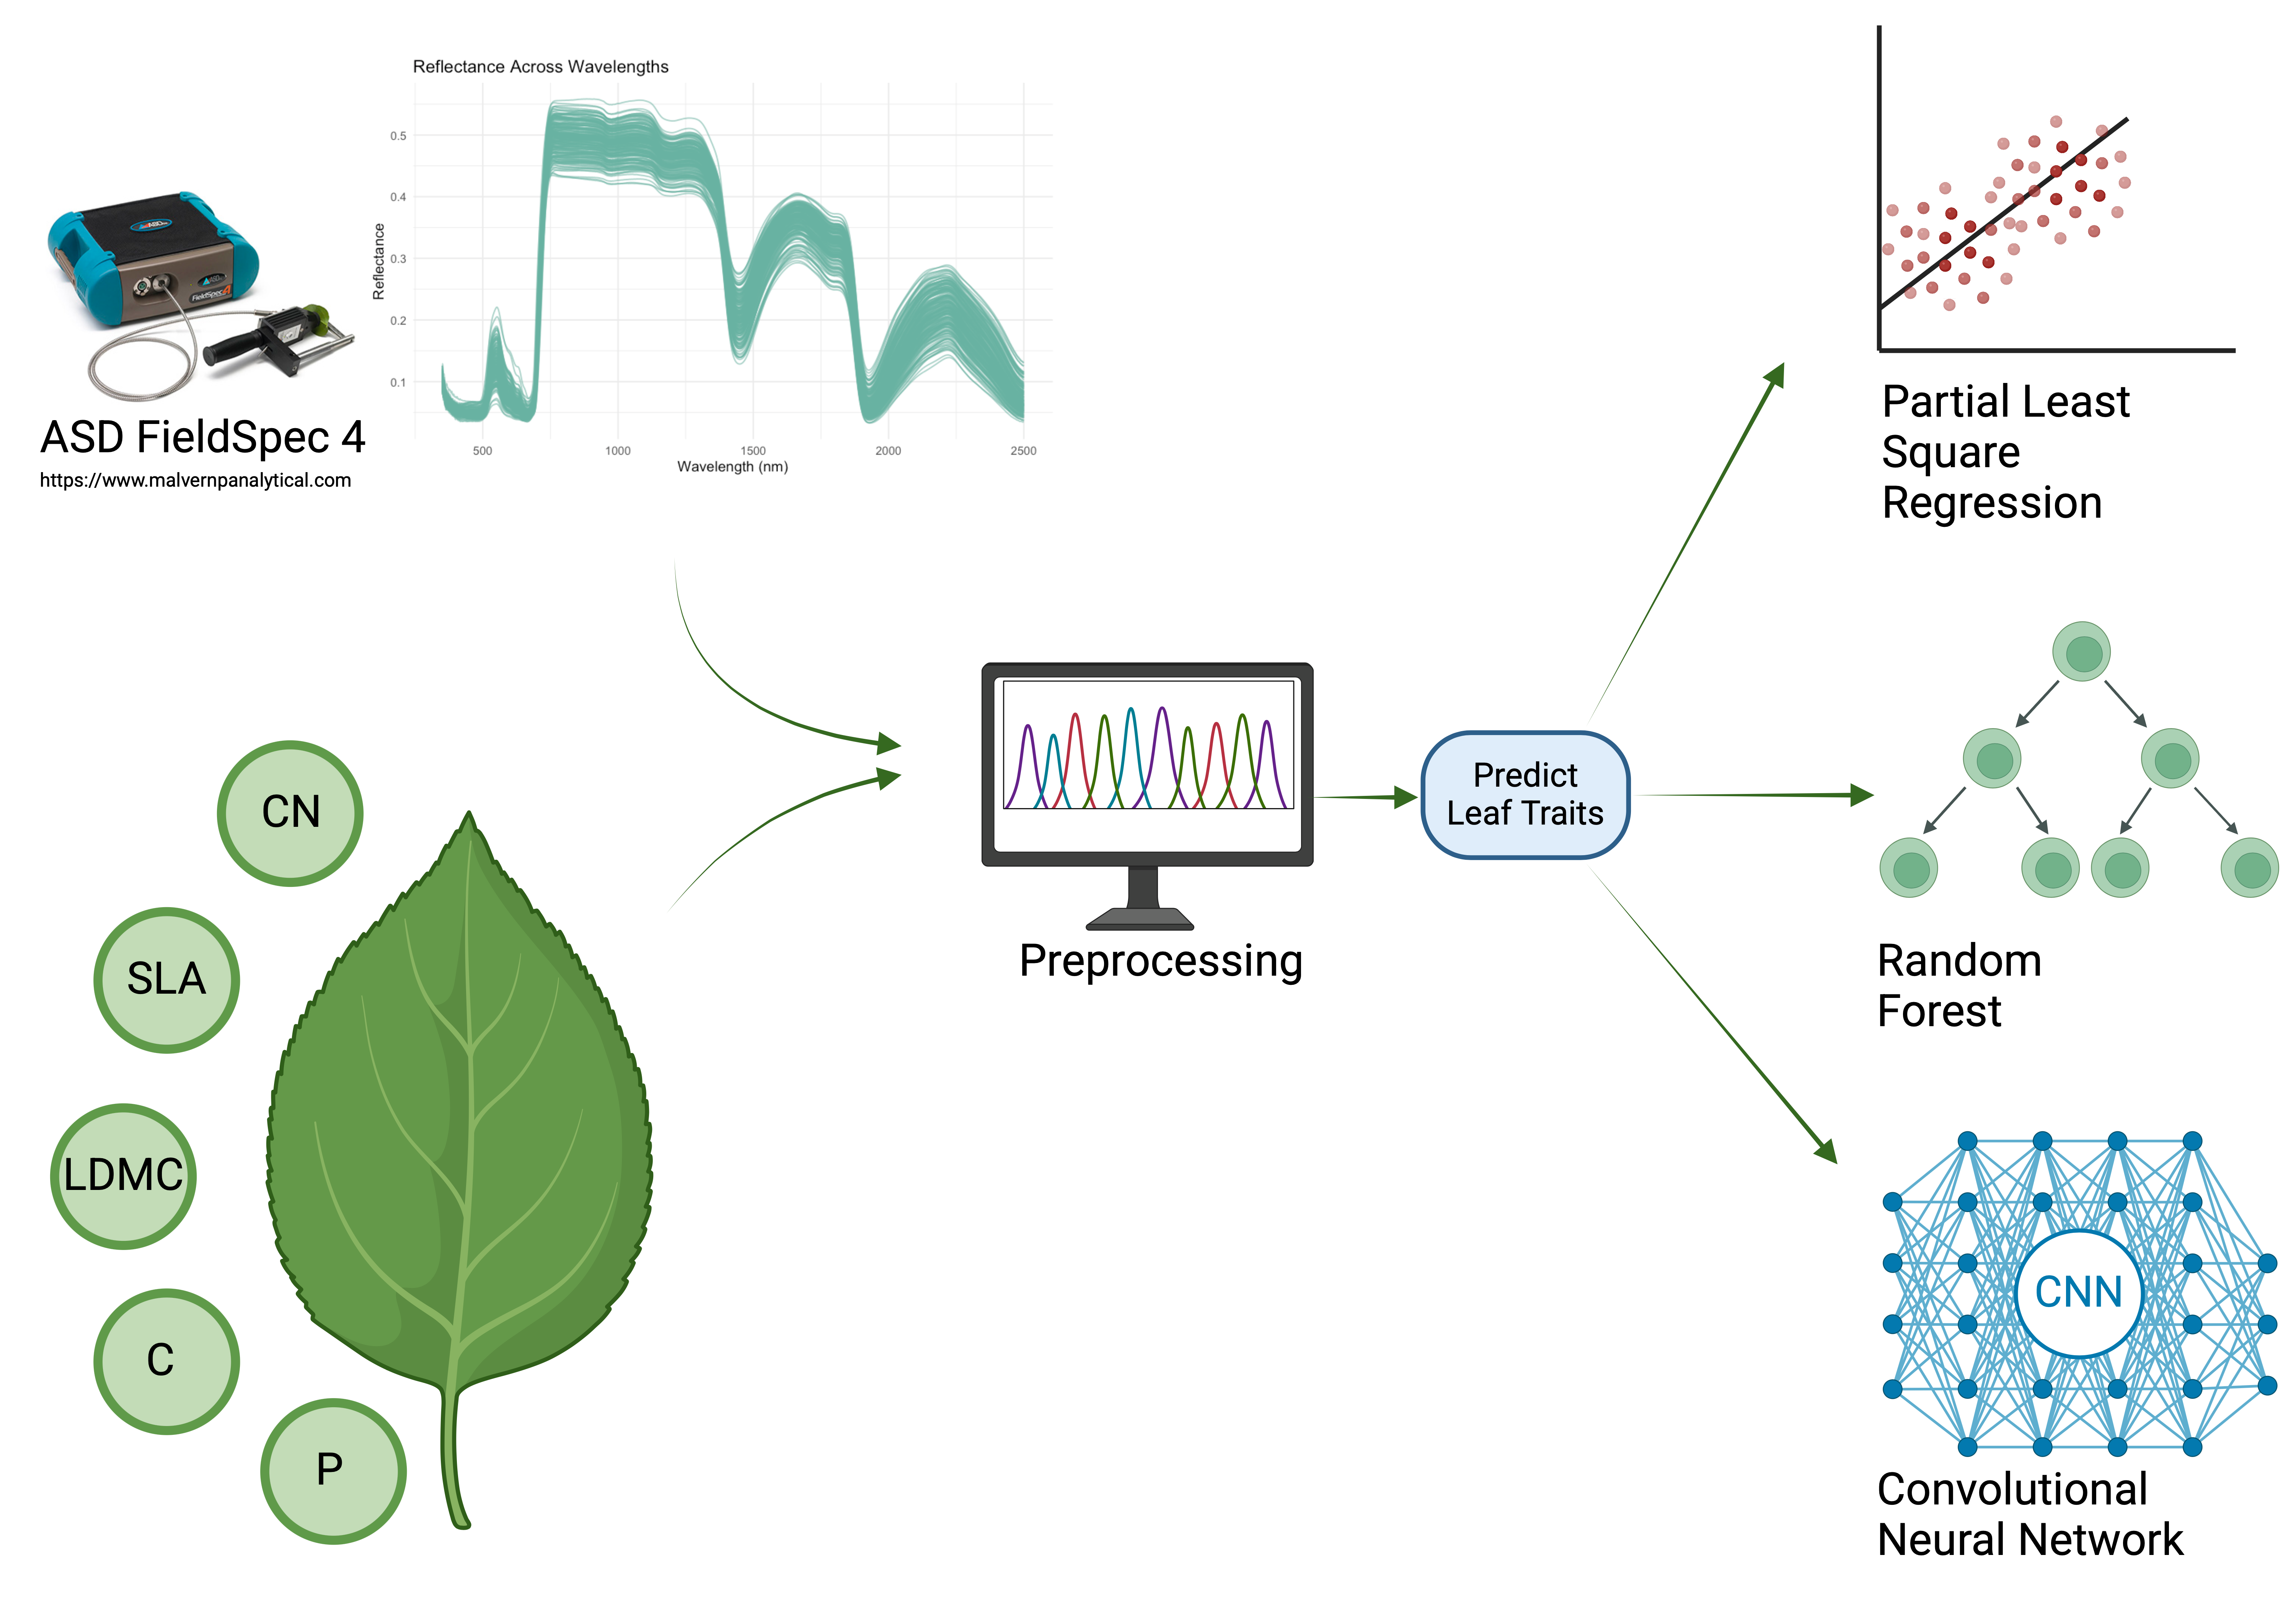
\includegraphics[width=0.6\textwidth]{Figures/nirs.png}
    \caption{A simplified workflow displying the process of trait prediction from NIRS data}
    \label{fig:nirs_workflow}
\end{figure}
Morphological and chemical traits were determined, including:
\begin{itemize}
    \item Specific Leaf Area (SLA)  $\text{mm}^2/\text{mg}$
    \item Leaf Dry Matter Content (LDMC)  $\text{mg}/\text{g}$
    \item Carbon-to-Nitrogen ratio (C:N)  $\text{g}/\text{g}$
    \item Carbon content (C)  $%$ 
    \item Phosphorus content (P) $\mu\text{mol}/\text{g}$
\end{itemize}
    

\subsubsection*{Trait Prediction Using Machine Learning}


\subsection{LCMS Feature Prediction From NIRS Data}
\subsubsection*{Background of the study}
\subsubsection*{LCMS feature prediction using Machine Learning}
\section{HPC runs}


\chapter{Results and Discussion}



\begin{table}[h!]
\centering
\caption{\textcolor{darkblue}{Comparison of 3 ML models across data}}
\label{tab:main-sub-table}
\begin{tabular}{lccc}
\toprule
\multicolumn{4}{c}{\textbf{\textcolor{darkblue}{Partial Least Square Regression (PLSR)}}} \\ 
\midrule
\textbf{Trait} & \textbf{$R^2$} & \textbf{RMSE} & \textbf{Training time} \\
\midrule
SLA  & 0.89 & 0.40 & 13.76 sec \\
LDMC & 0.85 & 0.41 & 11.40 sec \\
C:N  & 0.72 & 0.50 & 15.71 sec \\
C    & 0.68 & 0.55 & 13.63 sec \\
P    & 0.66 & 0.64 & 15.19 sec \\
\midrule
\multicolumn{4}{c}{\textbf{{PLSR Extrapolation}}} \\ 
\midrule
SLA (H 30\%) & 0.14 & 1.06 &  21.07 sec \\
SLA  (L 30\%)& 0.70 & 0.93 &  52.38 sec \\
\midrule
\multicolumn{4}{c}{\textbf{\textcolor{darkblue}{Random Forest (RF)}}} \\ 
\midrule
\textbf{Trait} & \textbf{$R^2$} & \textbf{RMSE} & \textbf{Training time} \\
\midrule
SLA  & 0.87 & 0.42 & 12.85 min \\
LDMC & 0.54 & 0.72 & 12.11 min \\
C:N  & 0.57 & 0.63 & 12.60 min \\
C    & 0.37 & 0.82 & 13.17 min \\
P    & 0.50 & 0.66 & 15.25 min \\
\midrule
\multicolumn{4}{c}{\textbf{{RF Extrapolation}}} \\ 
\midrule
SLA (H 30\%) & 0.035 & 1.29 &  11.64 min \\
SLA  (L 30\%)& 0.17 & 1.53 & 3.44 min \\
\midrule
\multicolumn{4}{c}{\textbf{\textcolor{darkblue}{Convolutional Neural Network (CNN)}}} \\
\midrule
\textbf{Trait} & \textbf{$R^2$} & \textbf{RMSE} & \textbf{Training time} \\
\midrule
SLA  & 0.89 & 3.69 & 28.11 min \\
LDMC & 0.88 & 0.11 & 30.20 min \\
C:N  & 0.74 & 6.26 & 4.11 min \\
C    & 0.36 & 4.31 & 4.83 min \\
P    & 0.20 & 43.42 & 31.30 sec \\
\bottomrule
\end{tabular}
\end{table}





\section{Data charecterestics}
histogram, spectra
\section{Baseline Machine Learning Models Pablo}
PLS, RF, CNN

\subsection{Variable importance}

\section{ Variations in Baseline systems}
\subsection{ modifying the Test and Training split}
\subsection{ input data length}

\section{Sues}

\chapter{Reference}

    
1. Pieruschka R, Schurr U. Plant Phenotyping: Past, Present, and Future. Plant Phenomics. 2019 Mar   26;2019:7507131. doi: 10.34133/2019/7507131. PMID: 33313536; PMCID: PMC7718630. \\
\\
2. Pulok K. Mukherjee, Quality control and evaluation of herbal drugs, Evaluating natural products and traditional medicine. 2019, doi:10.1016/C2016-0-042328, ISBN:978-0-12-813374-3. \\
\\
3. Nizamani, M. M., Zhang, Q., Muhae-Ud-Din, G., \& Wang, Y. (2023). High-throughput sequencing in plant disease management: A comprehensive review of benefits, challenges, and future perspectives. Phytopathology Research, 5(44). https://doi.org/10.1186/s42483-023-00215-7. \\
\\
4. Lane, H. M., \& Murray, S. C. (2021). High throughput can produce better decisions than high accuracy when phenotyping plant populations. Crop Science, 61(3), 1473–1484. https://doi.org/10.1002/csc2.20514. \\
\\
5. Zhang, N., Zhou, X., Kang, M., Hu, B.-G., Heuvelink, E., \& Marcelis, L. F. M. (2023). Machine learning versus crop growth models: An ally, not a rival. Journal of Experimental Botany, 74(4), 1259–1276. https://doi.org/10.1093/jxb/erac517. \\
\\
6. Zhu H. Big Data and Artificial Intelligence Modeling for Drug Discovery. Annu Rev Pharmacol Toxicol. 2020 Jan 6;60:573-589. doi: 10.1146/annurev-pharmtox-010919-023324. Epub 2019 Sep 13. PMID: 31518513; PMCID: PMC7010403. \\
\\
7. Kelsey Chetnik, Elisa Benedetti, Daniel P Gomari, Annalise Schweickart, Richa Batra, Mustafa Buyukozkan, Zeyu Wang, Matthias Arnold, Jonas Zierer, Karsten Suhre, Jan Krumsiek,  maplet: an extensible R toolbox for modular and reproducible metabolomics pipelines, Bioinformatics, Volume 38, Issue 4, February 2022, Pages 1168–1170, https://doi.org/10.1093/bioinformatics/btab741. \\
\\
8. Peng, Roger D. R programming for data science. Victoria, BC, Canada: Leanpub, 2016. \\
\\
9. www.bioconductor.org \\
\\
10. Kumar, R., Bohra, A., Pandey, A. K., Pandey, M. K., \& Kumar, A. (2017). Metabolomics for plant improvement: Status and prospects. Frontiers in Plant Science, 8, 1302. https://doi.org/10.3389/fpls.2017.01302. \\
\\
11. González-Domínguez, R., García-Barrera, T., \& Gómez-Ariza, J. L. (2014). Metabolite profiling for the identification of altered metabolic pathways in Alzheimer's disease. Journal of Pharmaceutical and Biomedical Analysis, 107, 75–81. https://doi.org/10.1016/j.jpba.2014.10.010. \\
\\
12. Liebal, U. W., Phan, A. N., Sudhakar, M., Raman, K., \& Blank, L. M. (2020). Machine learning applications for mass spectrometry-based metabolomics. Metabolites, 10(6), 243. https://doi.org/10.3390/metabo10060243. \\
\\
13. Vaillant, A., Beurier, G., Cornet, D., Rouan, L., Vile, D., Violle, C., \& Vasseur, F. (2024). NIRSpredict: a platform for predicting plant traits from near infra-red spectroscopy. BMC Plant Biology, 24(1), 1100. https://link.springer.com/article/10.1186/s12870-024-05776-0. \\
\\
14. Marr S, Hageman JA, Wehrens R, van Dam NM, Bruelheide H, Neumann S. LC-MS based plant metabolic profiles of thirteen grassland species grown in diverse neighbourhoods. Sci Data. 2021 Feb 9;8(1):52. doi: 10.1038/s41597-021-00836-8. PMID: 33563993; PMCID: PMC7873126. \\
\\
15. Sánchez-Bermejo, P. C., Monjau, T., Goldmann, K., Ferlian, O., Eisenhauer, N., Bruelheide, H., Ma, Z., \& Haider, S. (2024). Tree and mycorrhizal fungal diversity drive intraspecific and intraindividual trait variation in temperate forests: Evidence from a tree diversity experiment. Functional Ecology. https://doi.org/10.1111/1365-2435.14549. \\
\\
16. Renner, I.E., Fritz, V.A. Using Near-infrared reflectance spectroscopy (NIRS) to predict glucobrassicin concentrations in cabbage and brussels sprout leaf tissue. Plant Methods16, 136 (2020). https://doi.org/10.1186/s13007-020-00681-7. \\
\\
17. R. Schubert et al., "A White-Box Workflow for the Prediction of Food Content From Near-Infrared Data Based on Fourier-Transformation," 2023 13th Workshop on Hyperspectral Imaging and Signal Processing: Evolution in Remote Sensing (WHISPERS), Athens, Greece, 2023, pp. 1-5, doi: 10.1109/WHISPERS61460.2023.10430694. \\
\\
18. Choi RY, Coyner AS, Kalpathy-Cramer J, Chiang MF, Campbell JP. Introduction to Machine Learning, Neural Networks, and Deep Learning. Transl Vis Sci Technol. 2020 Feb 27;9(2):14. doi: 10.1167/tvst.9.2.14. PMID: 32704420; PMCID: PMC7347027.\\
\\
19. Pichler, M., \& Hartig, F. (2022). Machine learning and deep learning—A review for ecologists. Methods in Ecology and Evolution, 13(9), 1984–2000. https://doi.org/10.1111/2041-210X.14061. \\
\\
20. Ji, F., Li, F., Hao, D., Shiklomanov, A. N., Yang, X., Townsend, P. A., Dashti, H., Nakaji, T., Kovach, K. R., Liu, H., Luo, M., \& Chen, M. (2024). Unveiling the transferability of PLSR models for leaf trait estimation: Lessons from a comprehensive analysis with a novel global dataset. New Phytologist. https://doi.org/10.1111/nph.19807. \\
\\
21. Georgios Kourounis, Ali Ahmed Elmahmudi, Brian Thomson, James Hunter, Hassan Ugail, Colin Wilson, Computer image analysis with artificial intelligence: a practical introduction to convolutional neural networks for medical professionals, Postgraduate Medical Journal, Volume 99, Issue 1178, December 2023, Pages 1287–1294, https://doi.org/10.1093/postmj/qgad095. \\
\\
22. Liu S, Cheng H, Ashraf J, Zhang Y, Wang Q, Lv L, He M, Song G, Zuo D. Interpretation of convolutional neural networks reveals crucial sequence features involving in transcription during fiber development. BMC Bioinformatics. 2022 Mar 15;23(1):91. doi: 10.1186/s12859-022-04619-9. PMID: 35291940; PMCID: PMC8922751. \\
\\
23. van Dijk ADJ, Kootstra G, Kruijer W, de Ridder D. Machine learning in plant science and plant breeding. iScience. 2020 Dec 5;24(1):101890. doi: 10.1016/j.isci.2020.101890. PMID: 33364579; PMCID: PMC7750553. \\
\\
24. Deo, R. C. (2015). Machine Learning in Medicine. Circulation, 132(20), 1920–1930. https://doi.org/10.1161/CIRCULATIONAHA.115.001593. \\
\\
25. Angela C Burnett, Jeremiah Anderson, Kenneth J Davidson, Kim S Ely, Julien Lamour, Qianyu Li, Bailey D Morrison, Dedi Yang, Alistair Rogers, Shawn P Serbin, A best-practice guide to predicting plant traits from leaf-level hyperspectral data using partial least squares regression, Journal of Experimental Botany, Volume 72, Issue 18, 30 September 2021, Pages 6175–6189, https://doi.org/10.1093/jxb/erab295. \\
\\
26. Xin, Y., Sheng, J., Miao, M., Wang, L., Yang, Z., \& Huang, H. (2022). A review of imaging genetics in Alzheimer's disease. Journal of Clinical Neuroscience, 93, 1-9. https://doi.org/10.1016/j.jocn.2022.04.017. \\
\\
27. Dormann, C. F., Elith, J., Bacher, S., \& Buchmann, C. M. (2013). Collinearity: A review of methods to deal with it and a simulation study evaluating their performance. Ecography, 36(1), 27-46. https://doi.org/10.1111/j.1600-0587.2012.07348.x. \\
\\
28. Wold, S., Esbensen, K., \& Geladi, P. (1987). Principal component analysis. Chemometrics and Intelligent Laboratory Systems, 2(1-3), 37-52. https://doi.org/10.1016/0169-7439(87)80084-9. \\
\\
29. Couronné, R., Probst, P. \& Boulesteix, AL. Random forest versus logistic regression: a large-scale benchmark experiment. BMC Bioinformatics 19, 270 (2018). https://doi.org/10.1186/s12859-018-2264-5.\\
\\
30. Schonlau, M., \& Zou, R. Y. (2020). The random forest algorithm for statistical learning. The Stata Journal, 20(1), 3-29. DOI: 10.1177/1536867X20909688. \\
\\
31. Liu X, Wu D, Zewdie GK, et al. Using machine learning to estimate atmospheric Ambrosia pollen concentrations in Tulsa, OK. Environmental Health Insights. 2017;11. doi:10.1177/1178630217699399. \\
\\
32. Yamashita, R., Nishio, M., Do, R.K.G. et al. Convolutional neural networks: an overview and application in radiology. Insights Imaging 9, 611–629 (2018). https://doi.org/10.1007/s13244-018-0639-9.\\
\\
33. Alzubaidi, L., Zhang, J., Humaidi, A.J. et al. Review of deep learning: concepts, CNN architectures, challenges, applications, future directions. J Big Data 8, 53 (2021). https://doi.org/10.1186/s40537-021-00444-8. \\
\\
34. Reyad, M., Sarhan, A. \& Arafa, M. A modified Adam algorithm for deep neural network optimization. Neural Comput \& Applic 35, 17095–17112 (2023). https://doi.org/10.1007/s00521-023-08568-z.\\
\\
35. Zhang W, Kasun LC, Wang QJ, Zheng Y, Lin Z. A Review of Machine Learning for Near-Infrared Spectroscopy. Sensors. 2022; 22(24):9764. https://doi.org/10.3390/s22249764. \\
\\
36. Sohn SI, Pandian S, Oh YJ, Zaukuu JZ, Kang HJ, Ryu TH, Cho WS, Cho YS, Shin EK, Cho BK. An Overview of Near Infrared Spectroscopy and Its Applications in the Detection of Genetically Modified Organisms. Int J Mol Sci. 2021 Sep 14;22(18):9940. doi: 10.3390/ijms22189940. PMID: 34576101; PMCID: PMC8469702.\\
\\
37. Ihaka, R. (2017). The r project: A brief history and thoughts about the future. Univ. Auckl, 4, 22. https://www.stat.auckland.ac.nz/~ihaka/downloads/Otago.pdf. \\
\\
38. Ndaba, S. (2023). A Review of the Use of R Programming for Data Science Research in Botswana. International Journal of Database Management Systems, 15(1), 16. https://doi.org/10.5121/ijdms.2023.15101. \\
\\
39. Venables, W. N., \& Smith, D. M. (2003). An introduction to R: notes on R: a programming environment for data analysis and graphics, version 1.9. 1. CRID: 1130282269082172544, ISBN: 0954161742, https://cir.nii.ac.jp/crid/1130282269082172544. \\
\\
40. www.malvernpanalytical.com \\
\\
41. www.spectravista.com \\
\\
42. Lantz, B. (2019). Machine learning with R: expert techniques for predictive modeling. Packt publishing ltd. \\
\\
43. Allwood, J. W., \& Goodacre, R. (2010). An introduction to liquid chromatography–mass spectrometry instrumentation applied in plant metabolomic analyses. Phytochemical Analysis: An International Journal of Plant Chemical and Biochemical Techniques, 21(1), 33-47. https://doi.org/10.1002/pca.1187. \\
\\
44. Breiman, L. (2001). Random Forests. Machine Learning, 45(1), 5–32. https://doi.org/10.1023/A:1010933404324 \\
\\
45. Chomal, V. S., \& Saini, J. R. (2015). Software project documentation-an essence of software development. International Journal of Advanced Networking and Applications, 6(6), 2563.\\
\\
46. Blischak, J. D., Davenport, E. R., & Wilson, G. (2016). A quick introduction to version control with Git and GitHub. PLoS computational biology, 12(1), https://doi.org/10.1371/journal.pcbi.1004668\\
\\


\end{document}